\documentclass[oneside,12pt]{book}
\usepackage{amssymb}
\usepackage{amsmath}
\usepackage{graphicx}
\usepackage{epsfig}
\usepackage[spanish]{babel}
\decimalpoint
\usepackage[latin1]{inputenc}
\usepackage{makeidx}
\usepackage{graphicx}
\usepackage{wrapfig}
\setlength{\topmargin}{-0mm} \setlength{\textwidth}{143mm}
\setlength{\textheight}{215mm} \setlength{\oddsidemargin}{15mm}
\setlength{\evensidemargin}{15mm}
\newcommand{\be}{\begin{equation}}
\newcommand{\ee}{\end{equation}}
\newcommand{\ba}{\begin{array}}
\newcommand{\ea}{\end{array}}
\newcommand{\matFrit}{\left(\begin{array}{lcr} 0 & A & 0 \\ A^{\ast} & 0 & B\\ 0 & B^* & C\end{array}\right)}
\newcommand{\matFritti}{\left(\begin{array}{lcr} 0 & A & 0 \\ A^{\ast} & D & B\\ 0 & B^* & C\end{array}\right)}
\newcommand{\gme}{\ensuremath{{SU(2)_L\times U(1)_Y}}}
\newcommand{\et}{\ensuremath{\hat e_{\theta}}}
\newcommand{\vevh}{\ensuremath{\langle\Phi\rangle_0}}
\newcommand{\mpi}{\ensuremath{\left(\ba{lr} 0 & 1 \\ 1 & 0 \ea\right)}}
\newcommand{\mpii}{\ensuremath{\left(\ba{lr} 0 & -i \\ i & 0 \ea\right)}}
\newcommand{\mpiii}{\ensuremath{\left(\ba{lr} 1 & 0 \\ 0 & -1 \ea\right)}}
\newcommand{\fcp}{\ensuremath{\mathop{\rightarrow}\limits^{CP}}}

\newtheorem{theorem}{Teorema}

\title{\vspace{-2cm}{\LARGE {\bf Universidad de Sonora}}\\ 
{\large Divisi\'on de Ciencias Exactas y Naturales\\ Departamento de F\'isica}\\
\vspace{4cm}
Texturas para las matrices de masa de los quarks fenomenol\'ogicamente
viables\\ \vspace{3cm}}
\author{{\small Tesis que para obtener el t\'itulo de}\\ 
{\small Licenciado en F\'isica}\\{\small presenta}\\
Braulio Joel Rojas Mayoral\vspace{3cm}} 
\date{{\small Febrero de 2011}}
\makeindex
\begin{document}
\maketitle
\pagenumbering{roman}
\tableofcontents
\renewcommand\tablename{Tabla}
\listoftables

{\normalsize
\chapter*{Agradecimientos}

Agradezco al Dr. Ezequiel Rodr\'iguez J\'auregui por haberme propuesto el tema
de tesis y por todo el tiempo que le dedic\'o.

Agradezco a mis sinodales Dra. Elena Tejeda, Dr. Ezequiel Rodriguez,
Dr. Roberto Duarte y M.C. Evaristo Rojas  por su ayuda en la mejora de la tesis.

A todos de los que aprend\'i y los que intentaron que aprendiera.

A mis amigos Paco, el primo, Boynas, Nahuel, Victor, Fany, la Kiry y la Qk, por
haber estado ah\'i. 

A la banda pesada (Ana, Anah\'i, Araceli, Chero, J. Monta\~no, Javieroso, Munga,
Oso y Vlady) por permitirme compartir con ellos la universidad y en particular
la banca.

A mi familia.

Gracias a Angelina por toda su incalculable ayuda.

A Erika por dejarme estar en su vida. 


\newpage}

{\normalsize
\chapter*{Dedicatoria}

A quien le sirva.

\newpage}

{\normalsize
\chapter*{Resumen}

En el presente trabajo se investiga la capacidad predictiva de cinco modelos de
texturas para las matrices de masa. La teor\'ia f\'isica con la que se calculan
los observables que se contrastan con los datos experimentales es el modelo
est\'andar electrod\'ebil. Los datos experimentales con los que se compara son
los modulos de la matriz de mezcla y  tres relacionados al fen\'omeno de
violaci\'on de $CP$.

Se usan algoritmos gen\'eticos para ajustarse a los datos experimentales de la 
mezcla de los quarks y la violaci\'on de $CP$. Mediante dicho ajuste se 
encuentran la matriz de mezcla de los quarks, los \'angulos internos del 
tri\'angulo unitario y el invariante de Jarlskog. El m\'etodo se implementa con
tres distintos conjuntos de intervalos de masa encontrados en la literatura 
calculados a energ\'ia de la masa del bos\'on $Z$ y cinco pares diferentes de
texturas para las matrices de masa. Se comparan los m\'odulos 
de los elementos de la matriz de mezcla y sus invariantes calculados contra
los reportados por Particle Data Group en el a\~no 2010, encontrando que 
\'unicamente una textura en las matrices de masa es compatible con toda la 
fenomenolog\'ia considerada. 
%Se pone a prueba la
%compatibilidad de las texturas y las masas con la suposic\'on del maximal en la
%violaci\'on de $CP$.

\newpage}



\linespread{1.75}{\normalsize
\setcounter{page}{1}
\pagenumbering{arabic}
\chapter{Introducci\'on}

%%%%%%%%%%%%%%%%%%%%%%%%%%%%%%%%%%%%%%%%%%%%%%%%%%%%%%%%%%%%%%%%%%%%%%%%%%%
\section{Justificaci\'on}
A pesar del enorme progreso experimental, el origen de la masa de los
fermiones es a\'un una pregunta fundamental no resuelta en f\'isica de 
part\'iculas. Generalmente, en el contexto del modelo est\'andar electrod\'ebil
(ME) las matrices de las masas de los quarks $M_u$ y $M_d$ son complejas (36 
par\'ametros reales), como se explica en el cap\'itulo 2, y tienen que ajustar 
diez par\'ametros f\'isicos: las seis masas de los quarks y los cuatro 
par\'ametros de la matriz unitaria de Cabibbo-Kobayashi-Maskawa, $V_{ckm}$, los
cuales son presentados en el cap\'itulo 3. El problema  tradicional del modelo 
de las matrices de masa de los quarks va m\'as all\'a del modelo est\'andar y
supone formas espec\'ificas para las matrices $M_{u,d}$ las cuales, despu\'es de
la diagonalizaci\'on, proporcionan los eigenvalores y los par\'ametros de 
mezcla. En el intento de entender la estructura del sabor escondida en la matriz
de masa de los fermiones se proponen texturas, que son matrices de masa con
algunos ceros impuestos a los elementos de matriz. Suponer que hay simetr\'ia
del sabor oculta en las texturas de las matrices de masa de los quarks podr\'ia
proporcionar sugerencias de la din\'amica en la generaci\'on de masa de los
quarks y de la violaci\'on de $CP$ (tema presentado en el cap\'itulo en el
cap\'itulo 2) en un marco te\'orico m\'as fundamental ~\cite{Fri200001}.
 Entonces, dadas las matrices $M_u$ y $M_d$, es esencial
distinguir ceros que no tengan contenido f\'isico de aquellos otros que implican
restricciones f\'isicas en el espacio de los par\'ametros. El reto de un modelo
de texturas es ajustarse correctamente a los datos experimentales.

En este trabajo se estudiar\'an algunas texturas en las matrices de masa que 
pueden reproducir satisfactoriamente al fen\'omeno de la mezcla de los quarks. 
En la literatura se ha mostrado ~\cite{Mah200901} que las texturas de Fritzsch 
con 6 ceros en las matrices de masa son totalmente descartables ya que no se
pueden obtener resultados que concuerden con los datos experimentales, mientras
que las texturas de 5 ceros de Fritzsch en las matrices de masa no pueden ser 
descartadas completamente. Con la intenci\'on de obtener un entendimiento de las
mezclas de los quarks surge el problema de encontrar la estructua de la textura 
m\'as simple que sea compatible con el fen\'omeno de mezcla de los quarks. En 
vista de la ausencia de una justificaci\'on te\'orica para las matrices de masa 
como las de Fritzsch, se vuelve esencial desde el punto de vista 
fenomenol\'ogico considerar matrices de masa diferentes a las de Fritzsch, tanto
para los quarks como para los leptones.

Con la mejora en la precisi\'on de los datos experimentales los modelos de cinco
y seis ceros tienen gran dificultad en ajustarse a los datos ~\cite{Bra199902}. 
Usando criterios de naturalidad y simplicidad Fritzsch y Xing ~\cite{Fri200001} 
encontraron desfavorables a los modelos III y V de las texturas de
Robert, Ramond y Ross ~\cite{rrr} las cuales se muestran en la tabla ~\ref{t2}.
Con los datos experimentales disponibles en el a\~no 2008 se encontr\'o que 
ninguna textura de seis ceros puede reproducir los datos experimentales y que la
\'unica de cinco ceros que s\'i puede es la textura de Fritzsch con la matriz de
masa del sector $u$ con dos ceros y el sector $d$ con tres ceros 
~\cite{Mah200901}. Las texturas anteriores se proponen sin ninguna 
consideraci\'on f\'isica m\'as alla de la busqueda de modelos que reproduzcan 
los datos experimentales. Una suposici\'on f\'isica que puede ser impuesta a las
texturas, con la intenci\'on de obtener un modelo de ceros consistente con tal 
suposici\'on, es el maximal en el invariante de Jarlskog; dicha suposici\'on se 
explica en el cap\'itulo 3.

%%%%%%%%%%%%%%%%%%%%%%%%%%%%%%%%%%%%%%%%%%%%%%%%%%%%%%%%%%%%%%%%%%%%%%%%%%%%%
\section{Matrices de masa}
La densidad lagrangiana del modelo est\'andar electrod\'ebil (ME), que es el 
tema del siguiente cap\'itulo, puede ser expresada con cuatro t\'erminos  
\be\label{lme3f}
\mathcal{L}_{ME}=\mathcal{L}_{din}+\mathcal{L}_b+\mathcal{L}_{\Phi}
+\mathcal{L}_{Yuk},
\ee
los cuales representan las densidades lagrangianas de los fermiones, de los 
bosones, del campo de Higgs y la de Yukawa, respectivamente. Los dos primeros 
t\'erminos proporcionan las interacciones, existentes en el ME, de los bosones 
de norma con los fermiones, adem\'as de los t\'erminos cin\'eticos de ambos. 
Para prorcionar masa a los bosones y fermiones se agrega el tercer y cuarto
t\'ermino, la densidad lagrangiana del campo de Higgs, $\Phi$, y la de Yukawa.
En el modelo est\'andar el mecanismo de Higgs es el responsable de que los 
campos de norma y los fermiones adquieran masa ~\cite{Gri198701}. Despu\'es del 
rompimiento de simetr\'ia, la lagrangiana de Yukawa proporciona masa a los 
fermiones mediante el acoplo con el campo de Higgs, con lo que se obtienen las
masas de Dirac.

En la naturaleza existen tres generaciones de fermiones con id\'enticas 
caracter\'isticas, excepto la masa. En el ME no hay una explicaci\'on para 
esta propiedad. Los fermiones elementales conocidos est\'an divididos en 
dos categor\'ias, los quarks y los leptones. Una diferencia que los distingue 
es que los quarks participan en todas las interacciones (fuerte, 
electromagn\'etica, d\'ebil y gravitacional) mientras que los leptones no 
son afectados por la interacci\'on fuerte. En el ME de tres generaciones las 
masas de los quarks es una matriz compleja de 3 $\times$ 3, y cuya forma no es 
proporcionada por el ME, como se ver\'a en el pr\'oximo cap\'itulo.

En la base donde la teor\'ia es invariante de norma, los acoplos de Yukawa
no necesariamente son diagonales, por lo tanto los quarks no son estados 
propios de la masa ya que los t\'erminos de masa acoplan a una misma familia de
quarks de diferente generaci\'on. Cuando se pasa a una base donde la matriz 
de masa de los quarks es diagonal, la base de los quarks f\'isicos, las 
corrientes cargadas ya no son diagonales, los quarks $u$ y los quarks $d$  de 
diferentes generaciones se mezclan. La matriz no diagonal, responsable de la 
mezcla de los quarks, es la matriz de Cabibbo-Kobayashi-Maskawa, denotada como 
$V_{ckm}$, y es una manera de tener la violaci\'on de $CP$ en el modelo 
est\'andar.
 
La forma funcional de la matriz de mezcla se define como ~\cite{Rod200101} y 
~\cite{Koi200601}
\be
V_{ckm}=U^{u\dag}_LU^{d}_L=\left(\ba{ccc} V_{ud}&V_{us}&V_{ub}\\
V_{cd}&V_{cs}&V_{cb}\\ V_{td}&V_{ts}&V_{tb}\ea\right),
\ee
donde las matrices $U^q_L$ son las matrices que diagonalizan a las matrices de 
masa de los quarks $u$ y $d$, como se explica en el siguiente cap\'itulo.
%%%%%%%%%%%%%%%%%%%%%%%%%%%%%%%%%%%%%%%%%%%%%%%%%%%%%%%%%%%%%%%%%%%%%%%%%%%%
\section{Objetivo}
El objetivo del presente trabajo es poner a prueba la capacidad predictiva de
texturas en las matrices de masa para el sector de los quarks utilizando
algoritmos gen\'eticos. Para lograrlo primero se obtendr\'an los valores de los
m\'odulos de los elementos de la matriz de mezcla de los quarks en los
intervalos experimentales utilizando diferentes texturas. A las texturas con las
que se obtengan resusltados que se ajusten a los datos experimentales se les
probar\'a su compatibilidad con la hip\'otesis de maximal del invariante de
Jarlskog y se presentar\'an las matrices de masa con las que se obtengan
resultados de acuerdo con los datos experimentales. 


\newpage}

{\normalsize
{\chapter{Modelo Est\'andar}}
\section{Introducci\'on}
El modelo de las interacciones de las part\'iculas elementales hoy visto como 
est\'andar es el resultado de una larga construcci\'on y muchas contribuciones 
ingeniosas, entre las cuales las de  S.L. Glashow (1961), S. Weinberg (1967), y 
A. Salam (1967) son especialmente notables ~\cite{Giu200701}. En el marco del 
modelo est\'andar la materia del universo est\'a hecha de fermiones elementales 
interactuando a trav\'es de campos, de los cuales ellos son la fuente. Las 
part\'iculas asociadas con las interacciones de los campos son bosones. El 
modelo est\'andar describe las interacciones electromagn\'eticas, fuerte y 
d\'ebil de las part\'iculas elementales, y su construcci\'on fue guiada por un 
principio de simetr\'ia. La fuerza gravitacional no es incluida en el modelo
est\'andar.

En el presente trabajo se estudian las matrices de masa que mejor logren ajustar
la matriz de mezcla $V_{ckm}$ a los datos experimentales. La teor\'ia f\'isica
con la que se calcular\'an los observables te\'oricos que se contrastar\'an con 
los datos experimentales es el modelo est\'andar electrod\'ebil. Entre los datos
experimentales con los que se comparar\'a est\'an los producidos por el 
fen\'omeno de violaci\'on de $CP$, tema que se trata en la siguiente secci\'on y
para el cual se necesita la lagrangiana del modelo est\'andar. 

En esta secci\'on se presentan las partes que conforman a la densidad 
lagrangiana del modelo est\'andar, explicando brevemente su papel en \'este. Una
vez presentes las partes, la secci\'on 1 termina con la construcci\'on de la
densidad lagrangiana del modelo est\'andar y se comenta que los acoplos de los
campos de los quarks con los campos de norma y los acoplos de Yukawa tienen que
ser obtenidos del experimento, el modelo est\'andar no predice un valor para
ellos. En la primera
parte se hace una breve introducci\'on al modelo est\'anadar y la lagrangiana 
cin\'etica de los bosones de norma. En las dos siguentes partes se presentan el
resto de los t\'erminos de la lagrangiana, la lagrangiana din\'amica de los
fermiones y los t\'erminos de los que se obtienen los campos masivos. La
secci\'on acaba con la cuarta parte, en donde se generaliza lo visto en las tres
anteriores para poder obtener la lagrangiana del modelo est\'andar para tres
generaciones de quarks y leptones. 

\subsection{Lagrangiana cin\'etica de los bosones}
El modelo est\'andar de las interacciones fundamentales es la teor\'ia 
que describe las interacciones fuerte, d\'ebil y electromagn\'etica de las
part\'iculas elementales (quarks y leptones). El modelo est\'andar es una
teor\'ia de norma basada en el grupo de simetr\'ia $SU(3)_c\times\gme$ 
~\cite{Cot200701}. Es posible estudiar solamente la interacci\'on
 electrod\'ebil del modelo basada en el grupo de simetr\'ia
$SU(2)_L\times U(1)_Y$, esto se debe a que la simetr\'ia del color $SU(3)_C$
no se rompe, por lo que no se mezcla con el grupo \gme. Los grupos determinan
las interacciones y el n\'umero de bosones de norma
\footnote{Los bosones de norma son las part\'iculas encargadas de mediar las
interacciones.}, un bos\'on de norma por cada uno de los generadores del grupo,
el n\'umero y las propiedades de los bosones escalares y los fermiones es libre,
pero ellos deben transformarse de una forma definida por el grupo de simetr\'ia.
La parte electrod\'ebil tiene cuatro bosones de norma, tres de ellos tienen masa
y el otro no, que corresponden a los tres generadores del grupo $SU(2)_L$ y al 
generador del grupo $U(1)_Y$. La densidad lagrangiana del modelo est\'andar 
electrod\'ebil (ME) es la suma de las contribuciones de los fermiones 
($\mathcal{L}_f$) y los bosones de norma ($\mathcal{L}_b$)
\be\label{1.1}
\mathcal{L}=\mathcal{L}_f+\mathcal{L}_b.
\ee 
La densidad lagrangiana ~(\ref{1.1}) debe de cumplir con ciertas propiedades:
tiene que ser invariante local de transformaciones del grupo \gme, reproducir la
fenomenolog\'ia de la interacci\'on electrod\'ebil y, adem\'as, los fermiones y 
tres de los cuatro bosones de norma deben ser masivos. 

%Cualquier teor\'ia de part\'iculas elementales debe ser consistente con la 
%relatividad especial. La combinaci\'on de la mec\'anica cu\'antica, el 
%electromagnetismo y la relatividad especial da la ecuaci\'on de Dirac y la
%cuantizaci\'on de campos en teor\'ia cu\'antica de campos ~\cite{Cot200701}. 
El primer triunfo de la teor\'ia cu\'antica de campos es la electrodin\'amica
cu\'antica ~\cite{Cot200701}, la cual describe las interacciones del electr\'on
y el campo electromagn\'etico. El modelo est\'andar es una teor\'ia de
interacci\'on de campos. Para estudiar la fenomenolog\'ia se ve en la densidad
lagrangiana del modelo est\'andar que existen t\'erminos para cada una de las
interacciones. En el ME se unifican las interacciones electromagn\'eticas y
d\'ebil; la unificaci\'on significa que son dos diferentes manifestaciones de
una misma interacci\'on. 

En analog\'ia con la energ\'ia cin\'etica del fot\'on, los t\'erminos 
cin\'eticos para los bosones de norma son 
\be\label{bono}
\mathcal{L}_b=-\frac{1}{4}B_{\mu\nu}B^{\mu\nu}-\sum^3_{i=1}\frac{1}{4}
W^i_{\mu\nu}W^{i\mu\nu}
\ee
en donde $B_{\mu\nu}$ es el campo de fuerza para el campo de norma $U(1)_Y$ dado
por
\be\label{tf}
B_{\mu\nu}=\partial_{\mu}\hat B_{\nu}-\partial_{\nu}\hat B_{\mu}
\ee
y $W^i_{\mu\nu}$ es la generalizaci\'on de ~(\ref{tf}) para grupos no abelianos,
es decir
\be\label{tfw}
W^i_{\mu\nu}=\partial_{\mu}\hat W^i_{\nu}-\partial_{\nu}\hat W^i_{\mu}+g
\epsilon_{jki}\hat W^j_{\mu}\hat W^k_{\nu}.
\ee
y se expresan en t\'erminos de los tres bosones de norma del grupo $SU(2)_L$, 
$\hat {\bf W}_{\mu}$, y el bos\'on de norma de $U(1)_Y$, $B_{\mu}$ 
~\cite{Giu200701}.


%%%%%%%%%%%%%%%%%%%%%%%%%%%%%%%%%%%%%%%%%%%%%%%%%%%
\subsection{Lagrangiana din\'amica de fermiones}
La parte din\'amica de los fermiones se obtiene imponiendo la invariancia de 
norma a la ecuaci\'on de Dirac de un fermi\'on sin masa bajo transformaciones 
del grupo \gme ~\cite{Cot200701} la cual es
\be\label{ldf}
\mathcal{L}^{din}_f=\bar\psi_Ri\gamma^{\mu}D_{\mu}\psi_R\bar \psi_Li\gamma^{\mu}
D_{\mu}\psi_L.
\ee
donde para el grupo $\gme$ la derivada covariante $D_{\mu}$, la cual en las
teor\'ias de norma reemplaza a la derivada ordinaria $\partial_{\mu}$ en la
lagrangiana, tiene la forma
\be\label{dcme}
\hat D_{\mu}=\partial_{\mu}+ig_2{\vec\tau}\cdot\frac{\hat {\bf W}_{\mu}}{2}
+ig_1Y\frac{\hat B_{\mu}}{2},
\ee
para los dobletes de quiralidad izquierda L de $SU(2)$, y la forma
\be\label{dcme2}
\hat D_{\mu}=\partial_{\mu}+ig'Y\frac{\hat B_{\mu}}{2}
\ee
para los singletes de quiralidad derecha R.
En la ecuaci\'on ~(\ref{ldf}) se introdujo la notaci\'on de quiralidad de la 
ecuaci\'on de Dirac ~\cite{Cot200701}, donde $\psi$ es un espinor de Dirac de
cuatro componentes, las quiralidades definidas por
$$
\psi_R=\frac{1}{2}(1+\gamma^5)\psi\quad\psi_L=\frac{1}{2}(1-\gamma^5)\psi,
$$ 
$\bar\psi=\psi^{\dag}\gamma^0$, $\gamma^5=i\gamma^0\gamma^1\gamma^2\gamma^3$ y $\gamma^{\mu}$ con $\mu=0,1,2,3$
son las matrices de Dirac\footnote{Para una explicaci\'on detallada ver 
~\cite{Ait200401}, ~\cite{Cot200701} o ~\cite{Gri198701}.}. Sustituyendo
~(\ref{dcme}) y ~(\ref{dcme2}) en ~(\ref{ldf}) para la parte izquierda y
derecha, respectivamente, se obtienen los acoplos de los fermiones con los
bosones de norma, de aqu\'i se obtienen las interacciones electrod\'ebiles. Para
una familia de quarks, el t\'ermino de ~(\ref{ldf}) correspondiente a las partes
izquierdas de los espinores de los quarks tiene la forma 
\be
\mathcal{L}^{din,L}_f=\left(\bar u_L,\bar d_L\right)i\gamma^{\mu}
(\partial_{\mu}+ig_2{\vec\tau}\cdot\frac{\hat {\bf W}_{\mu}}{2}+ig_1Y
\frac{\hat B_{\mu}}{2})\left(\ba{c} u_L\\ d_L\ea\right),
\ee
donde el primer t\'emino de la derecha es la eciaci\'on de Dirac de part\'icula
libre y los t\'erminos restantes son los de interacci\'on con los campos de
norma, aqu\'i ${\vec \tau}$ son las matrices de esp\'in de Pauli siguientes
$$
\tau_1=\left(\begin{array}{lr} 0 & 1\\ 1 & 0 \end{array}\right) \qquad
\tau_2=\left(\begin{array}{lr} 0 & -i\\ i & 0 \end{array}\right) \qquad
\tau_3=\left(\begin{array}{lr} 1 & 0\\ 0 & -1 \end{array}\right).
$$
Los acoplos del espinor fermi\'onico con los campos de norma $\hat{\bf W}_{\mu}$
son
$$
g_2j^{\mu}_1W^1_{\mu}=\frac{g_2}{2}\left(\bar u_L,\bar d_L\right)
\gamma^{\mu}\tau_1\left(\ba{c}u_L\\ d_L\ea\right)W^1_{\mu},
$$
$$
g_2j^{\mu}_2W^2_{\mu}=\frac{g_2}{2}\left(\bar u_L,\bar d_L\right)
\gamma^{\mu}\tau_2\left(\ba{c} u_L\\ d_L\ea\right)W^2_{\mu}
$$
y
$$
g_2j^{\mu}_3W^3_{\mu}=\frac{g_2}{2}\left(\bar u_L,\bar d_L\right)
\gamma^{\mu}\tau_3\left(\ba{c} u_L\\ d_L\ea\right)W^3_{\mu},
$$
donde se observa que las dos primeras ecuaciones acoplan al bos\'on de norma
componentes distintos del doblete. Esta caracter\'istica juega un papel muy
importante en la violaci\'on de $CP$ y se explicar\'a en la siguiente secci\'on.

Utilizando las matrices de Pauli, ${\vec\tau\cdot}\hat{\bf W}_{\mu}$ toma la 
forma
$$
{\vec\tau\cdot}\hat{\bf W}_{\mu}
=\left(\begin{array}{lr} W^3_{\mu} & W^1_{\mu}-iW^2_{\mu}\\
W^1_{\mu}+iW^2_{\mu} & -W^3_{\mu} \end{array}\right),
$$
con lo cual las componentes de la corrientes del isoesp\'in d\'ebil pueden
expresarse de una manera compacta
\be\label{3cid}
{\bf J}^{\mu}=\frac{1}{2}\left(\bar u_L,\bar d_L\right)\gamma^{\mu}
\vec\tau\left(\ba{c} u_L\\ d_L\ea\right),
\ee
as\'i que la forma compacta de las corrientes de isoesp\'in d\'ebil acopladas a 
los campos de norma de $SU(2)_L$ toma la forma
\be\label{cnd}
g_2{\bf J}^{\mu}\hat{\bf W}_{\mu}=\frac{g_2}{2}\left(\bar u_L,d_L\right)
\gamma^{\mu}\vec\tau\left(\ba{c} u_L\\ d_L\ea\right)\hat{\bf W}_{\mu}.
\ee
Para el acoplo del espinor con el campo de norma $\hat B_{\mu}$ se utiliza la
relaci\'on de Gell-Mann-Nishijima para expresar la hipercarga en funci\'on de la
carga el\'ectrica y la tercera componente del isoesp\'in
\be\label{rgmn}
Q=\tau_3+\frac{Y}{2}
\ee
finalmente se tiene
\be\label{cyl}
\frac{g_1}{2}j^{\mu}_{Y,L}\hat B_{\mu}=g_1\left(\bar u_L,\bar d_L\right)
\gamma^{\mu}(Q-\tau_3)\left(\ba{c} u_L\\ d_L\ea\right)\hat B_{\mu}.
\ee
De igual manera, para la parte de quiralidad derecha de ~(\ref{ldf}) utilizando
~(\ref{dcme2}) se tiene
\be\label{cyr}
\frac{g_1}{2}j^{\mu}_{Y,R}\hat B_{\mu}=g_1\left(\bar u_R,\bar d_R\right)
\gamma^{\mu}(Q-\tau_3)\left(\ba{c} u_R\\ d_R\ea\right)\hat B_{\mu}.
\ee
Las ecuaciones ~(\ref{cyl}), ~(\ref{dcme2}) y la tercera componente de la 
corriente d\'ebil acoplan los bosones de norma a una misma componente del
doblete. Dividiendo la densidad lagrangiana din\'amica ~(\ref{ldf}) en dos, una
parte de interacci\'on y una parte cin\'etica, es posible expresarla utilizando 
 ~(\ref{cnd}), ~(\ref{cyl}) y ~(\ref{cyr}) como
\be\label{17}
\mathcal{L}^{din}_f=L^{cin}_f+g_2{\bf J}^{\mu}\hat{\bf W}_{\mu}
+\frac{g_1}{2}(j^{\mu}_{Y,R}+j^{\mu}_{Y,L})\hat B_{\mu}.
\ee
Todas las interacciones existentes en el ME de los bosones de norma con los 
fermiones est\'an presentes en ~(\ref{17}).


%%%%%%%%%%%%%%%%%%%%%%%%%%%%%%%%%%%%%%%
\subsection{Generaci\'on de masa}
Para proporcionar masa a los bosones y fermiones se utliza el mecanismo de
Higgs, con el cual se induce un rompimiento espont\'aneo de simetr\'ia.  
Hasta el momento los cuatro bosones de norma ($\hat{\bf  W}_{\mu}$ y $\hat 
B_{\mu}$) y los fermiones se mantienen sin masa. Para resolver esto se agrega
la energ\'ia cin\'etica y potencial (la densidad lagrangiana) del campo de 
Higgs, $\Phi$
\be\label{lhiggs}
\mathcal{L}_{\Phi}=(D_{\mu}\Phi)^{\dag}(D^{\mu}\Phi)-V(\Phi^{\dag}\Phi).
\ee
Despu\'es del rompimiento de simetr\'ia el campo de Higgs
proporciona masa a los bosones de norma. 

El campo de Higgs es un doblete de $SU(2)$
$$
\Phi=\left(\begin{array}{c}\phi^+\\ \phi^0\end{array}\right),
$$
con un valor de expectaci\'on del vac\'io dado por
$$
\langle\Phi\rangle_0=\left(\ba{c} 0\\ v
\ea\right)
$$
y con estados excitados de la forma
\be\label{vevhe}
\left(\ba{c} 0\\ v+\frac{h(x)}{\sqrt{2}}  \ea\right)
\ee
donde $h$ es el campo f\'isico del Higgs. La lagrangiana de Higgs debe de ser
invariante de norma localmente. Si el valor de expectaci\'on del vac\'io del
campo de Higgs no es invariante, se dice que hay un rompimiento espont\'aneo de 
simetr\'ia. 

Para que los fermiones obtengan masa se introduce un t\'ermino de interacci\'on
entre el campo de Higgs y los fermiones, que debe ser invariante de norma, 
respetar la simetr\'ia del grupo $\gme$ y del que se obtengan masas de Dirac. La
lagrangiana de Yukawa
\be\label{ly}
\mathcal{L}_{Yuk}=-G_{\psi}\left[(\psi^{\dag}_L\Phi)\psi_R+
\psi^{\dag}_R(\Phi^{\dag}\psi_L)\right],
\ee
cumple con las condiciones requeridas. Despu\'es del rompimiento de simetr\'ia, 
el campo de Higgs $\Phi$ da masa a los fermiones
$$
\mathcal{L}_{Yuk}=-vG_{\psi}\left[\psi^{\dag}_L\psi_R+
\psi^{\dag}_R\psi_L\right],
$$
y se reconoce la forma de las masas de Dirac
\be\label{jojojo}
m_{\psi}=vG_{\psi}.
\ee
En el modelo est\'andar el mecanismo de Higgs es el responsable de que los 
campos de norma y los fermiones adquieran masa. Los detalles aun son 
especulaci\'on pues la part\'icula de Higgs nunca se ha visto y el potencial de 
Higgs es completamente desconocido, ~(\ref{phdres}) es solo una propuesta 
~\cite{Gri198701}.
Con esto es posible hacer que la densidad lagrangiana del ME est\'e completa; 
se tienen todas las interacciones del ME, el fot\'on se mantiene sin masa, los
fermiones y tres bosones de norma adquieren masa.

%%%%%%%%%%%%%%%%%%%%%%%%%%%%%%%%%%%%%%%%%%%%%
\subsection{Modelo Est\'andar con tres familias}
Para obtener la lagrangiana del ME se trabajar\'a con seis dobletes de 
quiralidad izquierda L, tres corrspondientes a los leptones
\be
L_1\equiv\left(\ba{c} \nu_{eL}\\ e_L  \ea\right), \qquad
L_2\equiv\left(\ba{c} \nu_{\mu L}\\ \mu_L  \ea\right), \qquad
L_3\equiv\left(\ba{c} \nu_{\tau L}\\ \tau_L  \ea\right),
\ee
y tres correspondientes a los quarks
\be
Q_1\equiv\left(\ba{c} u_L\\ d_L  \ea\right), \qquad
Q_2\equiv\left(\ba{c} c_L\\ s_L  \ea\right), \qquad
Q_3\equiv\left(\ba{c} t_L\\ b_L  \ea\right), \qquad
\ee
y con los correspondientes singletes de quiralidad derecha R
$$
l_e\equiv e_R,\qquad
l_{\mu}\equiv \mu_R,\qquad
l_{\tau}\equiv \tau_R,\qquad
$$
$$
l_{\nu_e}\equiv \nu_{eR},\qquad
l_{\nu_\mu}\equiv \nu_{\mu R},\qquad
l_{\nu_\tau}\equiv \nu_{\tau R},\qquad
$$
$$
u_{1}\equiv u_R,\qquad
u_{2}\equiv c_R,\qquad
u_{3}\equiv t_R,\qquad
$$
$$
d_{1}\equiv d_R,\qquad
d_{2}\equiv s_R,\qquad
d_{3}\equiv b_R.\qquad
$$
La generalizaci\'on de la lagrangiana de Yukawa consta de dos partes, una 
lagrangiana para los quarks
\be\label{lygq}
\mathcal{L}^q_{Yuk}=-\sum_{ij}\left[Y^D_{ij}(Q_{i}^{\dag}\Phi)d_{j}+
Y^{D*}_{ij}d^{\dag}_{j}(\Phi^{\dag}Q_{i})\right]
-\sum_{ij}\left[Y^U_{ij}(Q_{i}^{\dag}\tilde\Phi)u_{j}+
Y^{U*}_{ij}u^{\dag}_{j}(\tilde\Phi^{\dag}Q_{i})\right],
\ee
donde $i,j=1,2,3$ por lo que $Y^q_{ij}$ son los nueve elementos de una matriz
compleja de $3\time 3$; y otra para los leptones
\be\label{lygl}
\mathcal{L}^l_{Yuk}=-\sum_{i\beta}\left[Y^e_{i\beta}(L_{i}^{\dag}\Phi)l_{\beta}+
Y^{e*}_{i\beta}l^{\dag}_{\beta}(\Phi^{\dag}Q_{i})\right]
-\sum_{i\alpha}\left[Y^{\nu}_{i\alpha}(L_{i}^{\dag}\tilde\Phi)l_{\alpha}+
Y^{\nu*}_{i\alpha}l^{\dag}_{\alpha}(\tilde\Phi^{\dag}L_{i})\right],
\ee
donde $\beta=e,\mu,\tau$ y $\alpha=\nu_e,\nu_{\mu},\nu_{\tau}$ y los acoplos de 
Yukawa son matrices complejas y arbitrarias; entonces, la lagrangiana de Yukawa
es
\be\label{lyg}
\mathcal{L}_{Yuk}=\mathcal{L}^q_{Yuk}+\mathcal{L}^l_{Yuk}.
\ee
La lagrangiana din\'amica de los fermiones ~(\ref{ldf}) para el ME es
%\be\label{ldg}
$$
\mathcal{L}_{din}=i\sum_{1,2,3}\left(\bar L_i\gamma^{\mu}D_{\mu}L_i+
\bar Q_i\gamma^{\mu}D_{\mu}Q_i+\bar d_i\gamma^{\mu}D_{\mu}d_i +
\bar u_i\gamma^{\mu}D_{\mu}u_i\right)
$$
\be\label{ldg}
+i\sum_{\alpha}\bar l_{\alpha}\gamma^{\mu}D_{\mu}l_{\alpha}+i\sum_{\beta}\bar 
l_{\beta}\gamma^{\mu}D_{\mu}l_{\beta}.
\ee



La densidad lagrangiana de ME para tres generaciones es la suma de 
~(\ref{ldg}), ~(\ref{bono}), ~(\ref{lhiggs}) y ~(\ref{lyg})
\be\label{lme3f}
\mathcal{L}_{ME}=\mathcal{L}_{din}+\mathcal{L}_b+\mathcal{L}_{\Phi}
+\mathcal{L}_{Yuk}.
\ee
En el ME no hay forma de predecir al valor de los acoplos de norma $g_1$ y 
$g_2$, tampoco de las masas de los fermiones, la forma de los acoplos de Yukawa
no es predicha por el modelo est\'andar, ni del bos\'on de Higgs ni
del acoplo cu\'artico. Todos estos datos tiene que obtenerse del experimento
y con ellos ajustar el modelo para que haga una reproducci\'on de la realidad lo
m\'as precisa posible. Hasta ahora se trabajo con la lagrangiana inavariante de norma, las matrices de masa de los fermiones no representan las masas f\'isicas,
para que representen las masas f\'isicas se deb pasar a la bases donde las
matrices son diagonales y los eigenvalores son las masas de los fermiones. Uno
de los fen\'omenos que debe reproducir la densidad lagrangiana ~(\ref{lme3f}) es
la violaci\'on de $CP$. En la siguiente secci\'on se presentan las reglas de
transformaci\'on de los campos y se prueba la simetr\'ia de las partes de 
~(\ref{lme3f}) ante dichas transformaciones.
%%%%%%%%%%%%%%%%%%%%%%%%%%%%%%%%%%%%%%%%%%%%%%%%%%%%%%%%%%%%%%%%%%%%%%%%%%%%%5
%%%%%%%%%%%%%%%%%%%%%%%%%%%%%%%%%%%%%%%%%%%%%%%%%%%%%%%%%%%%%%%%%%%%%%%%%%%
%%%%%%%%%%%%%%%%%%%%%%%%%%%%%%%%%%%%%%%%%%%%%%%%%%%%%%%%%%%%%%%%%%%%%%%%%%

\section{Violaci\'on de $CP$}
Las leyes de conservaci\'on en f\'isica son debidas a la invariancia de los
sistemas bajo transformaciones de simetr\'ia. La invariancia ante la paridad 
significa que la derecha y la izquierda no pueden ser definidas en una esencia 
absoluta. La ley de invariancia de la conjugaci\'on de carga significa que los 
experimentos en un mundo de antimateria dar\'an resulatados equivalentes que los
hechos en este mundo.

En f\'isica cl\'asica, la paridad no es afectada por la coordenada temporal, es 
decir, conmuta con los desplazamientos temporales $t\rightarrow t+\Delta 
t$. Siguiendo el principio de correspondencia, para pasar de mec\'anica 
cl\'asica a mec\'anica cu\'antica, se requiere la representaci\'on mec\'anico 
cu\'antica del operador $\cal P$ y de la traslaci\'on temporal, a trav\'es del 
operador  $e^{-i\mathcal{H}\Delta t}$, para reproducir esta caracter\'istica. El
operador $\cal P$ debe conmutar con el operador $\mathcal{H}$, ya que en la 
teor\'ia cu\'antica ellos conmutan, lo que significa que la paridad es una buena
simetr\'ia en la naturaleza. La paridad no es un simetr\'ia en las interacciones
d\'ebiles; los experimentos de los decaimientos nucleares $\beta$, $\pi^{\pm}$ y
$\mu^{\pm}$ demostraron la violaci\'on  de $P$ e invariancia de $C$ bajo las 
interacciones d\'ebiles, por lo que no se debe satisfacer el requerimiento de 
ser una buena simetr\'ia. Una conclusi\'on equivalente se obtiene para el 
operador $\mathcal{C}$. Entonces, los operadores $\mathcal{C}$ y $\mathcal{P}$ 
no son los mismos a los definidos en mec\'anica cu\'antica, por lo que para 
definir las reglas de transformaci\'on de $CP$ se utiliza la parte de la 
lagrangiana que debe respetar la simetr\'ia. Suponiendo que el electromagnetismo
es invariante ante transformaciones $C$ y $P$, como sugieren los experimentos, 
es posible definir las reglas de transformaci\'on a partir de la lagrangiana de 
la electrodin\'amica y extenderlas al resto de la lagrangiana electrod\'ebil. 


Para que la lagrangiana del ME sea consistente con los experimentos debe tener 
al menos un t\'ermino que viole la simetr\'ia discreta $CP$. Tomando lo anterior
en cuenta la lagrangiana completa puede ser escrita como la suma de dos 
t\'erminos
$$
\mathcal{L}=\mathcal{L}_{CP}+\mathcal{L}_R
$$
donde $\mathcal{L}_{CP}$ es la parte en la que se conserva $CP$ y ${\cal L}_R$
la parte que viola $CP$. La manera de incluir la violaci\'on de $CP$ es en la
 matriz de mezcla, la cual no puede obtenerse de la teor\'ia, sino de los datos
experimentales. La matriz de mezcla juega un papel importante en el presente 
trabajo, es la fuente de la mayor\'ia de los datos que se usan como criterio de
la consistencia de los modelos te\'oricos estudiados. Los modelos te\'oricos 
deben ajustar los m\'odulos de los elementos de la matriz de mezcla, los 
\'angulos internos de los tri\'angulos unitarios y el invariante de Jarlskog. 

En esta secci\'on se habla de la violaci\'on de $CP$, no se deducen las reglas
de transformaci\'on, pero se transforma a la lagrangiana del ME utilizando estas
reglas. 

%%%%%%%%%%%%%%%%%%%%%%%%%%%%%%%%%%%%%%%%%%%%%%%%%%%%%%%%%%%% 
\subsection{Transformaciones de $CP$ en la lagrangiana del ME}
Las reglas de transformaci\'on de $CP$, de los campos en la lagrangiana del ME, 
son definidas por la parte de la lagrangiana que conserva $CP$, y est\'an dadas 
en el cuadro 1.
\begin{table}[h!]\label{t1}
\caption{Transformaciones discretas de campos y lo campos bilineales de Dirac.}
$$\ba{c|ccccc}
Campo & P & T & C & CP & CPT\\ \hline
B^{\mu}&  &   &   & -B_{\mu}& \\
W^{1\mu}&W^1_{\mu}& & -W^{1\mu} & -W_{1\mu} & \\
W^{2\mu}&W^2_{\mu}& & W^{2\mu} & W_{2\mu} & \\
W^{3\mu}&W^3_{\mu}& & -W^{3\mu} & -W_{3\mu} & \\
W^{+\mu}& &   &   & -e^{i\xi_w}W^-_{\mu} & \\
W^{-\mu}& &   &   & -e^{-i\xi_w}W^+_{\mu} & \\
A^{\mu}&  &   &   & -A_{\mu}& \\
Z^{\mu} & &   &   & -Z_{\mu} & \\
h       & &   &   & h        & \\
\bar\psi\xi & \bar\psi\xi & \bar\psi\xi & \bar\xi\psi & \bar\xi\psi & 
\bar\xi\psi\\

\bar\psi\gamma_5\xi & -\bar\psi\gamma_5\xi & \bar\psi\gamma_5\xi & \bar\xi\gamma
_5\psi & -\bar\xi\gamma_5\psi & -\bar\xi\gamma_5\psi\\

\bar\psi\gamma^{\mu}\xi & \bar\psi\gamma_{\mu}\xi & \bar\psi\gamma_{\mu}\xi & 
-\bar\xi\gamma^{\mu}\psi & -\bar\xi\gamma_{\mu}\psi & -\bar\xi\gamma^{\mu}\psi\\

\bar\psi\gamma^{\mu}\gamma_5\xi & -\bar\psi\gamma_{\mu}\gamma_5\xi & \bar\psi
\gamma_{\mu}\gamma_5\xi & \bar\xi\gamma^{\mu}\gamma_5\psi & -\bar\xi\gamma^{\mu}
\gamma_5\psi & -\bar\xi\gamma^{\mu}\gamma_5\psi\\ %\hline
\ea $$\end{table}

En el presente trabajo solo se considera el sector hadr\'onico (los quarks); el 
sector lept\'onico puede ser tratado en manera similar, si los neutrinos son 
part\'iculas de Dirac. Para mostrar qu\'e  partes de la lagrangiana respetan
$CP$ (son invariantes ante la acci\'on conjunta de los operadores ${\cal C}$ y
${\cal P}$) y qu\'e condiciones se deben cumplir para que exista violaci\'on de 
$CP$, se trabaja con la lagrangiana despu\'es del rompimiento espont\'aneo de 
simetr\'ia, con campos de norma y quarks masivos, y al diagonalizar la matriz de
masa, con los campos de los quarks f\'isicos, ya que hay partes de la 
lagrangiana que no respetan la simetr\'ia cuando no se trabaja con los campos 
f\'isicos y s\'i es respetada por los campos f\'isicos ~\cite{Ber199701}. 

Primero se trabaja con los t\'erminos que no contienen a los campos de los 
fermiones. Tomando en cuenta que una lagrangiana pura de norma es invariante 
ante las transformaciones de $CP$ ~\cite{Gri199501}, se muestra que el t\'ermino
cin\'etico de los bosones de norma es invariante de $CP$. Aplicando las reglas 
de transformaci\'on del cuadro 1 a las ecuaciones ~(\ref{tf}) y ~(\ref{tfw})
$$B_{\mu\nu}=\partial_{\mu}\hat B_{\nu}-\partial_{\nu}\hat B_{\mu}$$
$$W^i_{\mu\nu}=\partial_{\mu}W^i_{\nu}-\partial_{\nu}W^i_{\mu}+g\epsilon_{jki}
W^j_{\mu}W^k_{\nu}$$
y observando que la derivada parcial se transforma bajo la acci\'on de 
${\cal CP}$ de la forma $\partial^{\mu}\rightarrow\partial_{\mu}$, se obtienen 
las transformaciones de los campos de fuerzas
\be\label{tcptf}
B^{\mu\nu}\fcp-B_{\mu\nu}
\ee
y
\be\label{tcptfw}
\left(W^1_{\mu\nu},W^2_{\mu\nu},W^3_{\mu\nu}\right)\fcp
-\left(W^{1\mu\nu},-W^{2\mu\nu},W^{3\mu\nu}\right).
\ee
Aplicando ~(\ref{tcptf}) y ~(\ref{tcptfw}) a la ecuaci\'on ~(\ref{bono}) se 
demuestra que la lagrangiana cin\'etica de los bosones es invariante ante la 
acci\'on de ${\cal CP}$

\be\label{invCPlb}
{\cal L}_b\fcp{\cal L}_b.
\ee

De manera equivalente para el sector del Higgs se observa que, despu\'es del 
rompimiento de simetr\'ia, el potencial de Higgs ~(\ref{phdres}) es invariante 
ante $CP$. Aplicando las reglas de transformaci\'on del cuadro 1 al resto de la
lagrangiana del Higgs ~(\ref{lh}) se muestra la invariancia de la lagrangiana
completa del Higgs
\be\label{invCPlh}
{\cal L}_{\Phi}\fcp{\cal L}_{\Phi}.
\ee
Los t\'erminos que no incluyen los campos de los fermiones son invariantes ante 
transformaciones de $CP$, el resto de los t\'erminos de la lagrangiana del ME 
~(\ref{lme3f}) involucran los campos f\'isicos de los fermiones (en particular
en este trabajo se estudiar\'a los campos de los quarks). Por lo anterior, la 
violaci\'on de $CP$ solo puede surgir de aquellos t\'erminos en los que est\'an 
presentes los campos f\'isicos de los quarks. 

Utilizando ~(\ref{vevhe}) y ~(\ref{jojojo}) en ~(\ref{lygq}) se obtiene la
lagrangiana de masa de los quarks, que son los t\'erminos de la lagrangiana de  
Yukawa despu\'es del rompimiento espont\'aneo de simetr\'ia que son 
proporcionales a $v$, y tiene la forma 
\be\label{lmq}
\mathcal{L}^q_{masa}=-\sum_{ij}\left[m^U_{ij}\bar u'_iu_j+m^{U*}_{ij}\bar u_j
u'_i\right]-\sum_{ij}\left[m^D_{ij}\bar d'_id_j+m^{D*}_{ij}\bar d_jd'_i\right],
\ee
en donde las $u_i$ son los singletes derechos de los quarks y los $u'_i$ son los
componentes de los dobletes izquierdos; las matrices de masa est\'an definidas 
por 
$$m^D_{ij}=vY^D_{ij}.$$
Aun no se est\'a trabajando con los campos f\'isicos de los quarks. Cuando se 
introdujo la lagrangiana de Yukawa se consider\'o que deb\'ia cumplir con 
ciertas condiciones de simetr\'ia (ser invariante de norma y respetar la 
simetr\'ia del grupo {\gme }), los acoplos de Yukawa, $Y^{U,D}$, m\'as generales
que cumplen con esas condiciones de simetr\'ia son matrices complejas. Para que 
los campos de los quarks $u_i$ representen campos f\'isicos, las matrices de 
masa deben ser diagonales y los valores de la diagonal ser las masas de los 
quarks, que se obtiene de los datos experimentales, recordando que en el ME no 
hay forma de predecir las masas de los fermiones. Como cualquier matriz 
cuadrada, sin importar si es hermitiana o no, puede ser diagonalizada mediante 
dos matrices unitarias, la matriz diagonal cuyos valores son las masas de los 
quarks es de la siguiente manera
\be\label{mdu}
U^{u\dag}_Lm^UU^{u}_R\equiv \mbox{diag}(m_u,m_c,m_t)
\ee
\be\label{mdd}
U^{d\dag}_Lm^DU^{d}_R\equiv \mbox{diag}(m_d,m_s,m_b).
\ee
Tal transformaci\'on es equivalente a cambiar los campos de los quarks de la
base de los eigenestados del sabor a la de los eigenestados de las masas, 
introduciendo acoplos no diagonales en la lagrangiana de las corrientes 
cargadas, en la cual solo las partes izquierdas est\'an involucradas.

Sustituyendo ~(\ref{mdu}) y ~(\ref{mdd}) en ~(\ref{lmq}) se obtiene 
\be\label{tlmq}
\bar u'_im^Uu_j=\bar u'mu=\bar u'U_LU^{\dag}_LmU_RU^{\dag}_Ru=
\overline{u^{fis}}'\mbox{diag}(m_u,m_c,m_t)u^{fis},
\ee
de donde los $u^{fis}_i$, los campos f\'isicos de los quarks tipo $u$ con masa
definida, son expresados de la siguiente manera

$$
u^{fis}_L=U^{q\dag}_L\left(\ba{c} u_L\\ c_L\\ t_L\ea\right).
$$
La lagrangiana de masa de los quarks f\'isicos es
$$
\mathcal{L}^{qf}_{masa}=-[m_u(\bar u_L^{fis}u_R^{fis}+
\bar u_R^{fis}u_L^{fis})]
-[m_d(\bar d_L^{fis}d_R^{fis}+\bar d_R^{fis}d_L^{fis})]
$$
\be\label{lmqf}
-[m_s(\bar s_L^{fis}s_R^{fis}+\bar s_R^{fis}s_L^{fis})]
-[m_c(\bar c_L^{fis}c_R^{fis}+\bar c_R^{fis}c_L^{fis})]
\ee
$$
-[m_b(\bar b_L^{fis}b_R^{fis}+\bar b_R^{fis}b_L^{fis})]
-[m_t(\bar t_L^{fis}t_R^{fis}+\bar t_R^{fis}t_L^{fis})],
$$ 
como de aqu\'i en adelante se trabajar\'a  con los campos de los quarks masivos 
se omitir\'a el super\'indice $fis$ a menos que se considere necesario para no
crear confusi\'on en la notaci\'on. Para mostrar que la lagrangiana de masa de
los quarks f\'isicos es invariante ante $CP$ se utilizan las reglas de 
transformaci\'on, mostradas en el cuadro 1, en el primer t\'ermino de 
~(\ref{lmqf}), obteniendo
$$
-[m_d(\bar d_Ld_R+\bar d_Rd_L)]\fcp-[m_d(\bar d_Rd_L+\bar d_Ld_R)]
$$
el resto de la lagrangiana ~(\ref{lmqf}) se transforman de manera 
equivalente. Los otros t\'erminos de la lagrangiana de Yukawa se trabajan igual,
utilizando la regla de transformaci\'on del campo de Higgs, por lo que se tiene
\be\label{incplY}
\mathcal{L}_{Yuk}\fcp\mathcal{L}_{Yuk}.
\ee

Para la parte din\'amica de la lagrangiana se hace un procedimiento equivalente.
Primero se trabaja con los t\'erminos de las corrientes neutras
$$
E\equiv i\bar u_LU^{u\dag}_L\gamma^{\mu}D_{\mu}U^{u}_Lu_L=i\bar u_L\gamma^{\mu}
\left[\partial_{\mu}+ig_2\tau_3\frac{\hat W^3_{\mu}}{2}
+ig_1Y\frac{B_{\mu}}{2}\right] u_L
$$
donde $u_L$, como ya se dijo, son los campos f\'isicos de los quarks $u$ de 
quiralidad izquierda. En la \'ultima igualdad se utiliz\'o la propiedad de las 
matrices unitarias, $U^{u\dag}_LU^u_L=1$. Dividiendo en tres partes a $E$,
expresando expl\'icitamante la matriz absorbida por la notaci\'on de la
quiralidad y aplicando las transformaciones de $CP$ se tiene
$$
E_1\equiv i\bar u\gamma^{\mu}\partial_{\mu}(1-\gamma^5)u\mathop{\rightarrow}
\limits^{CP}
(-i)\left[(-\bar u\gamma_{\mu}\partial^{\mu}u)-(-\bar u\gamma_{\mu}
\partial^{\mu}\gamma^5u)\right]
$$
$$
E_2\equiv \bar u\gamma^{\mu}g_2\frac{\hat W^3_{\mu}}{2}(1-\gamma^5)u
\fcp -\bar u\gamma_{\mu}g_2\left(\frac{-\hat W^{\mu}_3}{2}\right)(1-\gamma^5)u
$$
en donde hace falta un t\'ermino igual para los quarks tipo $d$ pero con signo 
contrario para $E_2$, causado por la tercera matriz de Pauli, $\tau_3$, y
$$
E_3\equiv \bar u\gamma^{\mu}g_1\left(\frac{2}{3}\right)\frac{B_{\mu}}{2}
(1-\gamma^5)u\fcp
-\bar u\gamma_{\mu}g_1\left(\frac{-B^\mu}{3}\right)(1-\gamma^5)u,
$$
con lo que se muestra la invariancia de los t\'erminos de las corrientes neutras
ante transformaciones de $CP$.

El \'ultimo t\'ermino del que puede surgir la violaci\'on de $CP$ es la parte de
las corrientes cargadas de la lagrangiana din\'amica ~(\ref{ldg}). Las 
corrientes cargadas son las \'unicas que restan por demostrar su invariancia. 
Como las corrientes cargadas solo involucran quarks parte izquierda, las 
matrices de los campos de los quarks f\'isicos parte derecha, $U^d_R$ y $U^d_R$,
no aparecen en las corrientes cargadas. El t\'ermino que falta transformar es de
las corrientes cargadas, que corresponde a las dos primeras componentes del
segundo t\'ermino, el de los quarks, de la ecuaci\'on ~(\ref{ldg})

$$
X_c\equiv[\hat W^1_{\mu}-i\hat W^2_{\mu}]\bar u_L\gamma^{\mu}U^{u\dag}_LU^d_Ld_L
+[\hat W^1_{\mu}+i\hat W^2_{\mu}]\bar d_L\gamma^{\mu}U^{d\dag}_LU^u_Lu_L,
$$
en donde la multiplicaci\'on de las matrices $U^{u\dag}_LU^d_L$ no 
necesariamente es la identidad. Aplicando las transformaciones de $CP$ a $X_c$ 
se obtiene
$$
X_c=[\hat W^1_{\mu}-i\hat W^2_{\mu}]\bar u_{\alpha}\gamma^{\mu}V_{\alpha j}
(1-\gamma_5)d_j+[\hat W^1_{\mu}+i\hat W^2_{\mu}]\bar d_j\gamma^{\mu}
V^*_{\alpha j}(1-\gamma_5)u_{\alpha}
$$
$$
\fcp[-\hat W^{1\mu}+i\hat W^{2\mu}](-\bar d_j\gamma_{\mu}V_{\alpha j}
(1-\gamma_5)u_{\alpha})+[-\hat W^{1\mu}-i\hat W^{2\mu}](-\bar u_{\alpha}
\gamma_{\mu}V^*_{\alpha j}(1-\gamma_5)d_j).
$$
As\'i, para que se conserve $CP$ la matriz $V_{ckm}=U^{u\dag}_LU^{d}_L$ debe de 
ser real. La \'unica manera para que el ME sea consistente con los datos 
experimentales, relacionados a la violaci\'on de la simetr\'ia discreta $CP$, es
que la matriz $V_{ckm}$ sea compleja, ya que solo el t\'ermino de la lagrangiana
del ME que puede no respetar la simetr\'ia $CP$ es el de las corrientes 
cargadas. No hay manera que la violaci\'on de $CP$ venga de alg\'un otro 
t\'ermino, como ya se vio en ~(\ref{invCPlb}), ~(\ref{invCPlh}) y 
~(\ref{incplY}).

En el siguiente cap\'itulo se presentan las propiedades de la matriz $V_{ckm}$ y
la utilizaci\'on de los tri\'angulos unitarios y el invariante de Jarlskog para
el estudio del fen\'omeno de la violaci\'on de $CP$.





\newpage}

{\normalsize
\chapter{Fenomenolog\'ia}

%%%%%%%%%%%%%%%%%%%%%%%%%%%%%%%%%%%%%%%%%%%%%%%%%%%%%%%%%%%%%%%%%%%%%%%%%%%%%%%%
\section{Texturas}
Una teor\'ia m\'as fundamental que el modelo est\'andar deber\'ia permitir 
determinar $M_u$ y $M_d$ de una manera \'unica. Como las matrices de masa de los
quarks son de importancia fundamental es deseable obtener su estructura sin 
hacer suposiciones. El primer paso es determinar las matrices de masa a partir 
de datos experimentales. Evidentemente el paso anterior cuando mucho puede ser 
parcialmente exitoso, porque el conocimiento de los eigenvalores y los 
par\'ametros de mezcla no es suficiente para este prop\'osito. Un entendimiento 
profundo de la mezcla del sabor de los quarks y el fen\'omeno de la violaci\'on 
de $CP$, es deseable para estudiar las propiedades de las matrices de masa de 
los quarks $M_{u,d}$, cuyas texturas son totalmente desconocidas dentro del ME. 

Sin embargo, es posible hacer algunos progresos notando que las matrices de masa
pueden ser supuestas hermitianas, sin perder generalidad, para aquellas 
teor\'ias en las que no haya cambio de sabor en las corrientes de las parte 
derechas de los campos, como el modelo est\'andar. Como las partes 
derechas de los campos son singletes de $SU(2)$, siempre es posible escoger una 
base adecuada de los quarks parte derecha, que resulte en matrices de masa 
hermitianas. Una matriz de masa hermitiana general, $M_q$ (con $q=u $ o $ d$)
puede ser escrita como
$$
M_q=\left(\ba{ccc} E_q&A_q&F_q\\ A^*_q&D_q&B_q\\ F^*_q&B^*_q&C_q\ea\right),
$$
donde los elementos de la diagonal son reales y los elemento fuera de ella son
complejos.

En la mayor\'ia de los intentos por entender los modelos observados de las masas
y mezcla de los fermiones, se propone la existencia de una familia de simetr\'ia
abeliana o no abeliana, dejando una estructura especial del sabor en las 
matrices de Yukawa, que involucra texturas con ceros. En la b\'usqueda de las 
texturas de los ceros permitidos, se puede tomar la descripci\'on 
{\it bottom-up}, donde se usan los datos experimentales de las masas y mezcla de
los fermiones para derivar aquellas texturas de Yukawa que son permitidas por 
los experimentos.  

La textura con dos ceros de Fritzsch para la matriz hermitiana de masa de los 
quarks es 
\be
\label{matfrit}
{F2}=\matFritti,
\ee
como el elemento $V_{1,3}$ es el conjugado de $V_{3,1}$ ellos se cuentan como un
cero, y se puede obtener la textura con tres ceros de Fritzsch si se toma a 
$D=0$
\be\label{matfri}
{F3}=\matFrit,
\ee
donde $A$ y $B$ son elementos complejos y $C$ es un elemento real de la matriz 
de masas. Para obtener la textura de seis ceros de Fritzsch se toman matrices de
masa, tanto en el sector $u$ como en el $d$, de la forma de la matriz 
~(\ref{matfri}). Las texturas de cinco ceros se obtienen tomando el sector $u$ 
con la forma de ~(\ref{matfri}) o ~(\ref{matfrit}) y al sector $d$ con la forma 
de la matriz no escogida para el sector $u$, por lo tanto hay dos texturas de 
Fritzsch de cinco ceros.  

No existe ninguna justificaci\'on te\'orica para las matrices de masa  
propuestas por Fritzsch, por lo tanto, se vuelve esencial, desde el punto de 
vista fenomenol\'ogico, considerar matrices de masa de los quarks diferentes a 
las propuestas por Fritzsch ~\cite{Mah200901}. Las matrices diferentes a las de 
Fritzsch tienen los ceros en otros elementos de la matriz de masa. 
{\tiny
\begin{table}[h!]\label{t2}
\begin{scriptsize}
\caption{Matrices de { masa} hermitianas de los quarks con consistencia 
fenomenol\'ogica seg\'un Ramond, Robert y Ross ~\cite{rrr}.}
$$\ba{c|ccccc}\hline\hline
\mbox{ RRR} & I & II & III & IV & V\\ \hline \\
M_u&\left(\ba{ccc} 0&A&0\\ A*&D&0\\ 0&0&C \ea\right) & 
\left(\ba{ccc} 0&A&0\\ A*&0&B\\ 0&B*&C \ea\right) & 
\left(\ba{ccc} 0&0&F\\ 0&D&0\\ F*&0&C \ea\right) & 
\left(\ba{ccc} 0&A&0\\ A*&D&B\\ 0&B*&C \ea\right) & 
\left(\ba{ccc} 0&0&F\\ 0&D&B\\ F*&B*&C \ea\right)\\  \\ \hline\\
M_d&\left(\ba{ccc} 0&A&0\\ A&D&B\\ 0&B&C \ea\right) & 
\left(\ba{ccc} 0&A&0\\ A*&D&B\\ 0&B*&C \ea\right) & 
\left(\ba{ccc} 0&A&0\\ A*&D&B\\ 0&B*&C \ea\right) & 
\left(\ba{ccc} 0&A&0\\ A*&D&0\\ 0&0&C \ea\right) & 
\left(\ba{ccc} 0&A&0\\ A*&D&0\\ 0&0&C \ea\right)\\  \\ \hline
\ea $$
\end{scriptsize}
\end{table}
}
Ramond, Robert y Ross (RRR) ~\cite{rrr} propusieron matrices sim\'etricas o 
hermitianas para buscar estructuras en los acoplos de Yukawa de los quarks que 
estuvieran en acuerdo con los datos experimentales. En su investigaci\'on ellos
trabajaron con texturas de cinco y seis ceros y encontraron cinco texturas de
cinco ceros que eran consistentes con los experimentos, \'estas se muestran en
la tabla 3.1.
%~\ref{t2}.

\subsection{Maximal en el invariante de Jarlskog}
Aunque hay muchas versiones diferentes de la hip\'otesis del maximal en la 
violaci\'on de $CP$, la versi\'on convencional demanda que la naturaleza tome un
valor en la fase de la violaci\'on de $CP$ tal que el invariante de Jarlskog,
$J$, tome su valor m\'aximo ~\cite{Koi200401}.

Como en el modelo est\'andar solo hay una fuente de la violaci\'on de $CP$, que
es la fase $\delta$ de violaci\'on de $CP$, en consecuencia, todos los 
observables de la violaci\'on de $CP$ est\'an fuertemente correlacionados. Desde
el punto de vista de la teor\'ia fundamental de los quarks esta situaci\'on no
es satisfactoria y es de inter\'es ver el origen te\'orico de la fase $\delta$ 
de la matriz de mezcla. En el a\~no 2001 se hizo un trabajo ~\cite{Rod200101} 
con el prop\'osito de mostrar que el maximal en el invariante de Jarlskog, $J$, 
y el maximal en la fase de la violaci\'on de $CP$ son fenomenol\'ogicamente 
permitidos. El invariante de Jarlskog, $J$, est\'a relacionado a la violaci\'on 
de $CP$ y es funci\'on de la fases de violaci\'on, $\delta$. Es bien conocido 
que el invariante de Jarlskog $J$ se obtiene de las matrices de masa de los 
quarks $M_q$. A partir de imponer la condici\'on de maximal al invariante de 
Jarlskog y a la fase de la violaci\'on de $CP$ se obtiene que las matrices de 
Ramond que cumplen con dichas condiciones son los modelos I, III, IV y V 
~\cite{Rod200101}.


Normalmente se dice que cualquiera de las convenci\'ones de fase de la matriz de
Cabibbo-Kobayashis-Maskawa ($V_{ckm}$) son equivalentes entre s\'i, por la 
invariancia ante refasamiento. Esto es verdad para todas las cantidades 
observables. Sin embargo, las matrices de masa de los quarks ($M_u,M_d$) no son
invariantes de refasamiento, aunque \'estas son invariantes ante cambios de 
base: $M_u\rightarrow M'_u=A^{\dag}M_uB_u$, 
$M_d\rightarrow M'_d=A^{\dag}M_dB_d$. A veces la invariancia de refasamiento se
confunde con la invariancia de cambio de bases. El par\'ametro $\delta$ de la
violaci\'on de $CP$ en la mariz $V_{ckm}$ no es observable, y depende de la
convenci\'on de fase. Las cantidades observables relacionadas a la violaci\'on
de $CP$ son los \'angulos ($\phi_1, \phi_2,\phi_3$)=($\beta,\alpha,\gamma$) en los tri\'angulos unitarios. Cuando se
toma una convenci\'on de fases, el par\'ametro $\delta$ se vuelve observable.
Las predicciones  basadas en la hip\'otesis de m\'axima violaci\'on de $CP$ 
pueden ser obtenidas exitosamente solo cuando se adoptan las convenciones de 
fase original, de Kobayashi-Maskawa, y la de Fritzsch-Xing ~\cite{Koi200601}.

%%%%%%%%%%%%%%%%%%%%%%%
Por ejemplo, considerando una matriz de mezcla, $V_{ckm}$, dada como
\be\label{2.1}
V=V(i,j)\equiv R^T_iP_jR_jR_k\qquad (i\neq j\neq k),
\ee
donde las $R_i$ son definidas por
$$
R_1(\theta)=\left(\ba{ccc} 1&0&0\\0&c&s\\0&-s&c\ea\right), \qquad
R_2(\theta)=\left(\ba{ccc} c&0&s\\0&1&0\\-s&0&c\ea\right), \qquad
R_3(\theta)=\left(\ba{ccc} c&s&0\\-s&c&0\\0&0&1\ea\right), 
$$
con $s=\sen\theta$ y $c=\cos\theta$, y las $P_i$ est\'an dadas por 
$P_1=\mbox{diag}(e^{i\delta},1,1) $, $P_2=\mbox{diag}(1,e^{i\delta},1)$ y 
$P_3=\mbox{diag}(1,1,e^{i\delta})$, es posible obtener la convenci\'on de fase 
original, la convenci\'on de Kobayashi-Maskawa, a partir de $V(1,1)$
$$
V_{km}=R^T_1(\theta_2)P_3(\delta_{km}+\pi)R_3(\theta_1)R_1(\theta_3)
$$
\be\label{cfkm}
=\left(\ba{ccc}c_1&-s_1c_3&-s_1s_3\\ s_1c_2&c_1c_2c_3-s_2s_3e^{i\delta_{km}}&
c_1c_2s_3+s_2c_3e^{i\delta_{km}}\\
 s_1s_2&c_1s_2c_3+c_2s_3e^{i\delta_{km}}&c_1s_2s_3-c_2c_3e^{i\delta_{km}}
\ea\right),
\ee
entonces, la cantidad invariante $J$ est\'a dada por 
\be\label{invJcfkm}
J=c_1s^2_1c_2s_2c_3s_3\sen\delta_{km},
\ee
es decir
\be\label{1.19}
J=\frac{|V_{11}||V_{12}||V_{13}||V_{21}||V_{31}|}{1-|V_{11}|^2}\sen\delta_{km},
\ee
y se necesita, para obtener un maximal, que $\delta_{km}=\frac{\pi}{2}$.

%La convenci\'on de fase propuesta por Fritzsch y Xing en 1997 puede ser obtenida
%de la expresi\'on $V(3,3)$, y de forma expl\'icita est\'a dada por
%$$
%V(3,3)=R^T_3(\theta^u_{12})P_1(\delta)R_1(\theta_{23})R_3(\theta^d_{12})
%$$
%\be\label{v33}
%V(3,3)=\left(\ba{ccc} e^{i\delta}c^u_{12}c^d_{12}+c_{23}s^u_{12}s^d_{12}&
%e^{i\delta}c^u_{12}s^d_{12}-c_{23}s^u_{12}c^d_{12}&-s_{23}s^u_{12}\\
%e^{i\delta}s^u_{12}c^d_{12}-c_{23}c^u_{12}s^d_{12}&
%e^{i\delta}s^u_{12}s^d_{12}+c_{23}c^u_{12}c^d_{12}& s_{23}c^u_{12}\\
%-s_{23}s^d_{12}&-s_{23}c^d_{12}&c_{23}\ea\right).
%\ee
%Para la expresi\'on ~(\ref{v33}), se tiene la forma del invariante $J$ como
%\be\label{invJcffx}
%J=c_{23}s^2_{23}c^u_{12}s^u_{12}c^d_{12}s^d_{12}\sen\delta=
%\frac{|V_{13}||V_{23}||V_{33}||V_{32}||V_{31}|}{1-|V_{33}|^2}\sen\delta.
%\ee


%%%%%%%%%%%%%%%%%%%%%%%%%%%%%%%%%%%%%%%%%%%%%%%%%%%%%%%%%%%%%%%%%%%%%%%%%5
\section{Datos experimentales}
La \'unica manera para que el ME sea consistente con los datos experimentales, 
relacionados a la violaci\'on de la simetr\'ia discreta $CP$, es que la matriz
$V_{ckm}$ sea compleja, ya que el \'unico t\'ermino de la lagrangiana del ME
que puede no respetar la simetr\'ia $CP$ es el de las corrientes cargadas. 
La fenomenolog\'ia de las interacciones electrod\'ebiles asegura que la matriz 
$V_{ckm}$ es compleja y unitaria. $V_{ckm}$ puede ser parametrizada por nueve 
par\'ametros (o en general por $n^2_g$ par\'ametros, donde $n_g$ es el n\'umero 
de familias). Pero se sabe de la mec\'anica cu\'antica que la fase de una 
funci\'on de onda no es una cantidad medible; por este motivo, se debe examinar
cu\'ales fases son medibles y cu\'ales no tienen sentido f\'isico en la matriz 
de mezcla, $V_{ckm}$. Es posible absorber o cambiar cinco par\'ametros
($2n_g-1$) a partir de las fases de los quarks, adem\'as pueden ser 
parametrizados tres \'angulos de rotaci\'on ($\frac{1}{2}n_g(n_g-1)$), los 
\'angulos de Euler. As\'i, el resto de los par\'ametros de la matriz $V_{ckm}$,
a los que se les llaman fases, es uno ($n_{fase}=\frac{1}{2}(n_g-2)(n_g-1)$) y 
es esta fase la que proporciona la violaci\'on de $CP$ en el modelo est\'andar.
Esto no significa que la violaci\'on de $CP$ es entendida; solamente se ha 
encontrado una forma econ\'omica y fenomenol\'ogicamente exitosa de agregar la
violaci\'on de $CP$ en el modelo est\'andar ~\cite{Big200101}. Para dos familias
no es posible obtener violaci\'on de $CP$ con la descripci\'on que se acaba de
hacer, pero existen otros modelos con implicaciones de las cuales la violaci\'on
de $CP$ puede ser obtenida, por ejemplo, extendiendo el sector del Higgs la
violaci\'on de $CP$ es asociada al rompimiento espont\'aneo de simetr\'ia 
~\cite{Jar198901}.

Las cantidades con significado f\'isico deben ser invariantes bajo un cambio de
fase de los campos de los quarks; solo funciones de $V_{ckm}$ que sean 
invariantes ante refasamiento pueden ser medibles. Los invariantes m\'as simples
son los m\'odulos de los elementos de matriz, denotados por
$$U_{\alpha i}\equiv\left|V_{\alpha i}\right|^2.$$

Experimentalmente, las funciones invariantes ante cambio de fase de la matriz
$V_{ckm}$ para las cuales se tiene acceso m\'as directo, tambi\'en son los 
m\'odulos de sus elementos de matriz. Los valores experimentales actuales 
\cite{Nak201001} se presentan en la tabla 3.2.%~\ref{pdgvckm}.
{\tiny
\begin{table}[h!]\label{pdg}
\begin{scriptsize}
\caption{Valores experimentales de los m\'odulos de la matriz de mezcla.} 
$$\ba{c|c} \hline \hline
|V_{ckm}|&\mbox{Exp}\\ \hline
|V_{ud}|&0.97425\pm0.00022\\
|V_{us}|&0.2252\pm0.0009  \\
|V_{cd}|&0.230\pm0.011    \\
|V_{cs}|&1.023\pm0.036    \\
|V_{ub}|&(3.89\pm0.44)\times10^{-3} \\
|V_{cb}|&(40.6\pm1.3)\times10^{-3}  \\
|V_{td}|&(8.4\pm0.6)\times10^{-3}   \\
|V_{ts}|&(38.7\pm2.1)\times10^{-3}  \\
|V_{tb}|&0.88\pm0.07     \\ \hline
\ea
$$
\end{scriptsize}
\end{table}
}
%$$|V_{ud}|=0.97425\pm0.00022.$$ 
%Tres m\'etodos diferentes se han usado en su determinaci\'on, siendo el 
%estudio del decaimiento nuclear beta el m\'as preciso. La magnitud de $|V_{us}|$
%es tradicionalmente obtenido del decaimiento semilept\'onico del kaon; 
%tambi\'en es posible hacerlo a partir de los decaimientos lept\'onicos del kaon,
%del hiper\'on y del $\tau$. El valor promedio determinado es
%$$|V_{us}|=0.2252\pm0.0009$$
%La forma m\'as precisa para determina $|V_{cd}|$ esta basada en la 
%interacci\'on neutrino-antineutrino. El valor reportado es
%$$|V_{cd}|=0.230\pm0.011.$$
%Es posible determinar $|V_{cs}|$ de los decaimientos semilept\'onicos $D$ y 
%lept\'onicos $D_s$, siendo
%$$|V_{cs}|=1.023\pm0.036$$
%el valor. Los valor reportados para $|V_{cb}|$ y $|V_{ub}|$ se extraen de los 
%decaimiento $B$ y son
%$$|V_{ub}|=(3.89\pm0.44)\times10^{-3},$$
%$$|V_{cb}|=(40.6\pm1.3)\times10^{-3}.$$
%Los m\'odulos de la matriz de mezcla $|V_{td}|$ y $|V_{ts}|$ 
%no pude ser medidos del decaimiento a nivel de \'arbol del quark t, as\'i que se
%tienen que usar las oscilaciones $B^0_{d,s}-\bar B^0_{d,s}$, obteniendo
%$$|V_{td}|=(8.4\pm0.6)\times10^{-3}$$
%$$|V_{ts}|=(38.7\pm2.1)\times10^{-3}.$$
%La determinaci\'on directa de $|V_{tb}|$ se volvi\'o posible de la secci\'on 
%transversal en la producci\'on de quarks t, teniendo un valor
%de 
%$$|V_{tb}|=0.88\pm0.07.$$
Se observa que el valor central de $|V_{cs}|$ es mayor a 1, por lo tanto,
podr\'ia viola la unitariedad de la matriz de mezcla. Los elementos de la matriz
de mezcla pueden determinarse de mejor manera si adem\'as se utilizan las
restricciones impuestas por el ME. Las restricciones impuestas por la
unitariedad para tres generaciones reduce el intervalo permitido para los
elementos de la matriz de mezcla y son los siguientes ~\cite{Nak201001}
\be\label{pdgvckm}
|V_{ckm}|=\left(\ba{ccc} 0.97428\pm0.00015&0.2253\pm0.0007&
0.00347^{+0.00016}_{-0.00012}\\
0.2252\pm0.0007&0.97345^{+0.00015}_{-0.00016}&0.0410^{+0.0011}_{-0.0007}\\
0.00862^{+0.00026}_{-0.00020}&0.0403^{+0.0011}_{-0.0007}&0.999152^{+0.000030}
_{-0.000045}\ea\right).
\ee


Los siguientes invariantes, en orden de simplicidad, son los cuartetos,
$$
Q_{\alpha i\beta j}\equiv V_{\alpha i}V_{\beta j}V^*_{\alpha j}V^*_{\beta i},
$$
donde se pide que $\alpha\neq\beta$ y $i\neq j$, para que el cuarteto no se 
reduzca al producto de dos m\'odulos al cuadrado. En general, la violaci\'on de 
$CP$ existe si cualquiera de las funciones de $V_{ckm}$ invariantes ante
refasamiento no es real ~\cite{Bra199901}.

Como la matriz de mezcla de los quarks, $V_{ckm}$, es unitaria 
$$V_{ckm}V^{\dag}_{ckm}=V^{\dag}_{ckm}V_{ckm}=1$$
se pueden obtener seis relaciones de ortogonalidad, tres relaciones de pares de
renglones diferentes y tres de pares de diferentes columnas,
$$
V^{\dag}_{ckm}V_{ckm}= 
\left(\ba{ccc} V^*_{ud}&V^*_{cd}&V^*_{td}\\
V^*_{us}&V^*_{cs}&V^*_{ts}\\ V^*_{ub}&V^*_{cb}&V^*_{tb}\ea\right)
\left(\ba{ccc} V_{ud}&V_{us}&V_{ub}\\
V_{cd}&V_{cs}&V_{cb}\\ V_{td}&V_{ts}&V_{tb}\ea\right)
=\left(\ba{ccc} 1&0&0\\0&1&0\\0&0&1\ea\right),
$$
por ejemplo, del primer rengl\'on y la segunda columna se obtiene
\be\label{tu}
V_{ud}V^*_{cd}+V_{us}V^*_{cs}+V_{ub}V^*_{cb}=0.
\ee
Multiplicando a la ecuaci\'on ~(\ref{tu}) por $V^*_{us}V_{cs}$,
$$
V^*_{us}V_{cs}V_{ud}V^*_{cd}+V^*_{us}V_{cs}V_{us}V^*_{cs}+V^*_{us}V_{cs}V_{ub}
V^*_{cb}=0
$$
y tomando la parte imaginaria, se obtiene
$$ \mbox{Im}Q_{udcs}=-\mbox{Im}Q_{ubcs},$$
se concluye que los cuartetos $Q_{udcs}$ y $Q_{ubcs}$ tienen partes imaginarias
sim\'etricas. De manera equivalente, con el resto de los pares de renglones
diferentes y los pares de columnas diferentes, se concluye que la parte 
imaginaria de los cuartetos a lo m\'as difiere por un signo. De esta manera se
define el invariante de Jarlskog
\be\label{idj}
J\equiv \mbox{Im}Q_{uscb}=\mbox{Im}(V_{us}V_{cb}V^*_{ub}V^*_{cs}),
\ee
sabiendo que la parte imaginaria  de todos los cuartetos es igual a $J$, o con
signo distinto. El valor experimental para el invariante de Jarlskog es 
~\cite{Nak201001}
$$J=(2.91^{+0.19}_{-0.11})\times10^{-5}.$$

La relaci\'on de ortogonalidad ~(\ref{tu}) puede ser interpretada como un
tri\'angulo en el plano complejo. Sin embargo el tri\'angulo unitario que se usa
com\'unmente surge de la ecuaci\'on
\be\label{nanana}
V_{ud}V^*_{ub}+V_{cd}V^*_{cb}+V_{td}V^*_{tb}=0,
\ee
ver figura 3.1. Los 6 tri\'angulos,
uno por cada relaci\'on de ortogonalidad, son rotados cuando la matriz de mezcla
de los quarks, $V_{ckm}$, sufre un cambio de fase. Sin embargo, la forma de los
tri\'angulos permanece sin cambios, ya que los \'angulos internos y las
longitudes de los lados son invariantes ante el refasamiento.
%%%%%%%%%%%%%%%%%%%%%%%%%%%%%%%%%%%%%%%%%%%%%%%%%%5555
\begin{figure}\label{fig2}
\centering
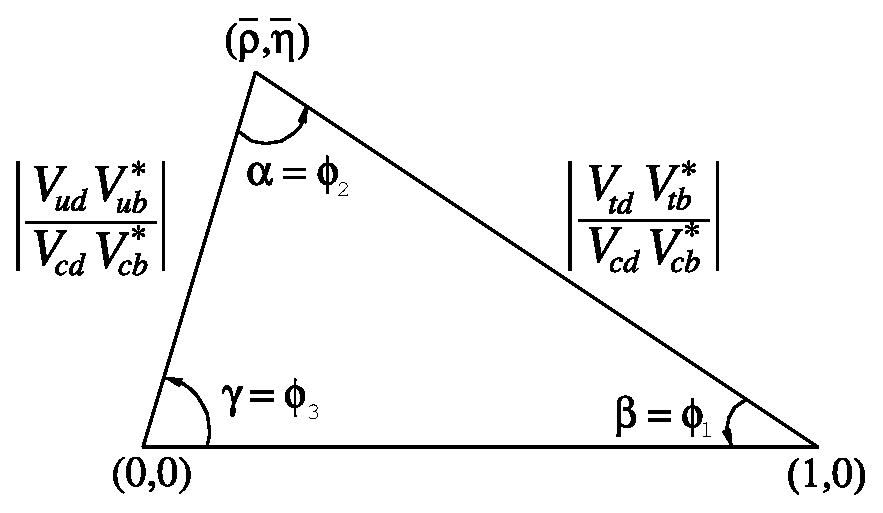
\includegraphics[height=8cm,angle=0]{triangle2.eps}
\caption{Tri\'angilo unitario en el plano complejo ~\cite{Nak201001}.}
\end{figure}
%%%%%%%%%%%%%%%%%%%%%%%%%%%%%%%%%%%%%%%%%%%%%%%%%%%%%%
Si se divide ~(\ref{nanana}) entre $V_{cd}V^*_{cb}$ se obtiene
$$
\frac{V_{ud}V^*_{ub}}{V_{cd}V^*_{cb}}+1+\frac{V_{td}V^*_{tb}}{V_{cd}V^*_{cb}}=0,
$$
en donde los \'angulos internos del tri\'angulo que se forma est\'an definidos 
como el argumento de n\'umeros complejos, dados de la siguiente manera
\be\label{alpha}
\alpha\equiv \mbox{arg}\left(-\frac{V_{td}V^*_{tb}}{V_{ud}V^*_{ub}}\right)
\ee
\be\label{beta}
\beta\equiv \mbox{arg}\left(-\frac{V_{cd}V^*_{cb}}{V_{td}V^*_{tb}}\right)
\ee
\be\label{gamma}
\gamma\equiv \mbox{arg}\left(-\frac{V_{ud}V^*_{ub}}{V_{cd}V^*_{cb}}\right),
\ee
y los valores experimentales son ~\cite{Nak201001}
$$\alpha=(88^{+6}_{-5}),$$
$$\sin{2\beta}=0.681\pm{0.025},$$
y
$$\gamma=77^{+30}_{-32}.$$

Una vez definidos los tri\'angulos, al invariante de Jarlskog se le 
puede dar la interpretaci\'on geom\'etrica del doble del \'area de los 
tri\'angulos
$$
A=\frac{|\mbox{Im} Q_{udcb}|}{2}=\frac{|J|}{2}. 
$$
As\'i, aunque los tri\'angulos tienen diferentes formas, el \'area de ellos es
la misma, $\frac{|J|}{2}$. Como los cuartetos son las funciones m\'as simples de
$V_{ckm}$ que pueden ser no reales, si $J$ es diferente de cero la violaci\'on 
de $CP$ existe, si es cero no hay violaci\'on y los tri\'angulos se colapsan a
una l\'inea y su \'area es cero.
%%%%%%%%%%%%%%%%%%%%%%%%%%%%%%%%%%%%%%%%%%%%%%%%%%%%%%%%%%%%%%%%%%%%%%%%%%%%%%%%
%%%%%%%%%%%%%%%%%%%%%%%%%%%%%%%%%%%%%%%%%%%%%
\subsection{Transformaciones de base d\'ebil, el trabajo de Branco y 
Emmanuel-Costa}

Branco y Emmanuel-Costa demostraron que siempre es posible hacer una 
transformaci\'on de base d\'ebil tal que las matrices de masa de los quarks sean
hermitianas y ambas presenten texturas de ceros en el elemento $(1,1)$, teniendo
la forma
\be\label{emI}
M_u=\left(\ba {lcr} 0&*&*\\ *&*&*\\ *&*&* \ea \right),\qquad 
M_d=\left(\ba {lcr} 0&*&*\\ *&*&*\\ *&*&* \ea \right).
\ee 
A partir de ~(\ref{emI}) intentaron llegar a texturas de cuatro ceros. Su 
motivaci\'on radicaba en el problema mostrado por las texturas de m\'as ceros 
en la reproducci\'on de datos fenomenol\'ogicos. La conclusi\'on a la que 
llegaron fue que en general no es posible obtener texturas de cuatro ceros a
partir de transformaciones de base d\'ebil, solo unas cuantas son accesibles.
Entre las texturas accesibles estaba aquella en la que ambas matrices de masa
ten\'ian ceros en $(1,1)$ y $(1,3)$, de la forma de las matrices con dos ceros
de Fritzsch ~(\ref{matfrit}) ~\cite{Bra199902}.

En trabajos posteriores Branco y colaboradores investigaron la dificultad que
presentaban algunas texturas al intentar determinar de manera precisa los 
\'angulos $\beta\equiv \mbox{arg}(-\frac{V_{cd}V^*_{cb}}{V^*_{td}V_{tb}})$ y
$\gamma\equiv \mbox{arg}(-\frac{V_{ud}V^*_{ub}}{V^*_{cd}V_{cb}})$ invariantes 
ante refasamiento ~\cite{Bra200401}. Una manera de resolver dicha discrepancia 
con los datos del \'angulo $\beta$ es proponer fases no factorizables, en al 
menos una matriz de masa. Para ellos la raz\'on era f\'acil de entender, la 
contribuci\'on de tal fase permit\'ia alcanzar los valores del $\sen2\beta$ 
demasiados grandes para la gran mayor\'ia de las texturas. Adem\'as, encontraron
la condici\'on necesaria para la existencia de fases no factorizables: las 
texturas no deben presentar ceros en elementos que no sean de la diagonal. Con 
esta condici\'on, ninguna textura de Fritzsch o las cinco propuestas por Ramond pueden presentar fases no factorizables. 

Siguiendo con la misma t\'onica, investigaron c\'omo los trabajos que 
propon\'ian nueva f\'isica afectaban a los datos que se utilizan como criterio
en la aceptaci\'on de alguna textura, en particular, otra vez, los \'angulos 
$\beta$ y $\gamma$. Su trabajo se bas\'o en texturas en las que no pudieran 
haber fases no factorizables. Clasificaron a las texturas dependiendo del 
\'angulo en el que presentaban problemas a la hora de reproducirlo. En el 
estudio del impacto de nueva f\'isica (NF) en las pruebas de las texturas de 
Yukawa, se tienen que especificar cu\'ales son la suposiciones de la naturaleza
de la NF. En la mayor\'ia de los escenarios de NF considerados en la literatura,
usualmente se asume que la NF no contribuye significativamente a  nivel de 
\'arbol en los decaimientos de {\it strange} y mesones $B$. Esto implica que la
NF no afecta los resultados de $|V_{su}|$, $|V_{cb}|$, $|V_{ub}|$ y $\gamma$ en
los datos experimentales. Utilizando estos cuatro datos, se puede reconstruir la
matriz de mezcla $V_{ckm}$ y los tri\'angulos unitarios. Sin embargo, se puede 
proponer que hay contribuciones apreciables por parte de la NF a las mezclas de
$B^0_d-\bar B^0_d$ y $B^0_s-\bar B^0_s$, as\'i los datos experimentales de 
$V_{td}$, $V_{ts}$ y $\beta$ son afectados. A la conclusi\'on que se llega en 
dicha investigaci\'on es que si una textura particular predice un valor de 
$\beta$ o de $|V_{td}|$ en desacuerdo con los datos experimentales, se puede 
justificar por la presencia de nueva f\'isica en la mezcla $B^0_d-\bar B^0_d$. 
Sin embargo, no se pueden justificar texturas que no den resultados correctos 
para $\frac{|V_{ub}|}{|V_{cb}|}$ o para $\gamma$. Esto es importante porque la 
mayor\'ia de las texturas de Yukawa tienen dificultad en obtener estos datos 
~\cite{Bra200601}.

En un trabajo m\'as reciente ~\cite{Emm200901} se concluy\'o que no es posible 
obtener texturas de cuatro ceros a partir de transformaciones de base d\'ebil.
Partiendo de ~(\ref{emI}) es posible agregar un cero extra al sector $d$ sin
modificar los ceros exactos de las texturas. Observando que a\'un hay un 
excedente de par\'ametros, se intenta obtener otro cero a partir de 
transformaciones de base d\'ebil, como ya se hab\'ia hecho a\~nos atras 
~\cite{Bra199902}, pero tomando en cuenta los datos experimentales recientes. 
Con \'estos, hicieron una variaci\'on aleatoria de todos los posibles valores 
permitidos de las masas de los quarks y los cuatro par\'ametros de la matriz de
mezcla $V_{ckm}$. Entonces, encontraron que tal transformaci\'on no es posible,
as\'i que la suposici\'on de cualquier cero adicional tiene implicaciones 
f\'isicas. Se pueden derivar todos los pares de $M_u$ y $M_d$ (quince pares en
total) que tienen un cero en la misma posici\'on en la diagonal para ambos 
sectores  y un cero adicional en el sector $d$. Tambi\'en se pudiera tener un
cero extra en el sector $u$ en lugar de el sector $d$, teniendo un total de
treinta pares de texturas de ceros de base d\'ebil ~\cite{Emm200901}. Ya que no
existe ninguna justificaci\'on para  
imponer que las matrices de masa sean hermitianas, tambi\'en obtuvieron que 
el n\'umero m\'aximo de ceros en las matrices de masa no hermitianas, que pueden
ser obtenidas a partir de transformaciones de bases d\'ebil, son nueve. Fritzsch
ya hab\'ia propuesto texturas de ceros a matrices de masa no hermitianas 
clasific\'andolas en tres tipos: interacci\'on de vecinos cercanos, matrices 
tri\'angular y matrices de fase ~\cite{Fri200001}. 


%%%%%%%%%%%%%%%%%%%%%%%%%%%%%%%%%%%%%%%%%%%%%%%%%%%%%%%%%%%%%%%%%%%%%%%%%5
\section{Metodolog\'ia}
Las masas de los quarks son los eigenvalores de la matriz de masa de los quarks,
las cuales son introducidas en el modelo est\'andar por el acoplo de los campos
de los quarks con el campo escalar. En el presente trabajo se utilizan tres 
diferentes c\'alculos de los intervalos de las masas a escala electrod\'ebil y 
son presentadas en la tabla 3.3.
%~\ref{t3masas}. 
Estos valores se utilizan para 
calcular la matriz $V_{ckm}$ te\'orica que se obtiene al diagonalizar texturas
en las matrices de masa de los quarks y deben compararse los datos 
experimentales de la mezcla de los quarks y la violaci\'on de $CP$.
\begin{table}[h!]\label{t3masas}
\begin{footnotesize}
\caption{ Intervalos de las masas de los quarks predichos a escala
electrod\'ebil, $M_Z$, reportados por Xing (2008), Emmanuel-Costa (2009) y Koide
(1997).}
$$\ba{c|ccc|}\hline\hline
 &\mbox{Xing }(M_Z) &\mbox{Emmanuel-Costa }(M_Z) &\mbox{Koide }(M_Z)\\ \hline 
m_u & 0.00127^{+0.00050}_{-0.00042}&0.0014^{+0.0006}_{-0.0005}&0.00233^
{+0.00045}_{-0.00042}\\
m_d & 0.0029^{+0.00125}_{-0.00119} & 0.0028\pm{0.0007} & 0.00469^{+0.0060}
_{-0.0066} \\
m_s & 0.055^{+0.015}_{-0.016} & 0.060^{+0.015}_{-0.019} & 0.0934^{+0.0118}
_{-0.0130} \\
m_c & 0.619\pm{0.084} & 0.64^{+0.07}_{-0.09} & 0.677^{+0.056}_{-0.061}\\
m_b & 2.89\pm{0.09} & 2.89^{+0.17}_{-0.08} & 3\pm{0.11} \\
m_t & 171.1\pm{3} & 170.1\pm{2.3} & 181\pm{13} \\ \hline
\ea $$
\end{footnotesize}
\end{table}

La estructura de la matriz de mezcla, $V_{ckm}$, est\'a relacionada con la 
matriz de masas de los quarks. En este trabajo se considera que la matriz de 
masa es hermitiana, es posible expresarla de la forma 
\be 
M_q=P^{\dag}_q\tilde M_qP_q, 
\ee
donde $P_q$ son las matrices de fase diagonal 
\be\label{matfase}
P_q=\left(\ba{ccc}e^{if_{1q}}&0&0\\0&e^{if_{2q}}&0\\0&0&
e^{if_{3q}}\ea\right),
\ee
y $\tilde M_q$ son matrices reales sim\'etricas. Las matrices $\tilde M_q$ son 
diagonalizadas por matrices ortogonales $O_q$ como
\be\label{matsim}
O^{\dag}_q\tilde M_qO_q=\mbox{diag}(m_{q1},-m_{q2},m_{q3}),
\ee
entonces, la matriz de mezcla $V_{ckm}$ est\'a dada por 
\be\label{supuni}
V_{ckm}=O^T_uPO_d,
\ee 
donde $P=P^{\dag}_{u}P_{d}$. 

%Las masas de los quarks son \'unicamente 
%determinadas por la matriz $\tilde M_q$.  

Los modelos puestos a prueba en este trabajo son la textura de cinco ceros de 
Fritzsch, donde la matriz de masa del sector $u$ presenta dos ceros 
~\cite{Mah200901} y el sector $d$ tres ceros ~\cite{Mah200901}, y donde el 
sector $d$ es el que presenta la textura de 2 ceros de Fritszch y el sector $u$ 3 ceros la cual coincide con la segunda
textura propuesta por Ramond. Adem\'as de las texturas propuestas por Ramond y 
colaboradores se revisan los modelos I y IV, ya que son los que coinciden 
seg\'un el criterio de simplicidad y naturalidad ~\cite{Fri200001} y que pueden 
presentar maximal en el invariante de Jarlskog ~\cite{Rod200101}. Las texturas 
de cuatro ceros que se estudian son las propuestas por Fritzsch 
~\cite{Fri200201}, en donde ambos sectores presentan matrices con dos ceros de 
la forma ~(\ref{matfrit}) y la propuesta por Branco y Emmanuel-Costa donde el 
sector $u$ es una matriz real y en el sector $d$ es compleja, ambas con la forma
~(\ref{matfrit}) ~\cite{Bra199902}. 

Para obtener la matriz de mezcla se tienen que diagonalizar las matrices de 
masa, un paso esencial en el proceso de diagonalizaci\'on es considerar a los 
invariantes $Tr(\tilde M_q)$, $\chi^2(\tilde M_q)$ y $det(\tilde M_q)$ los 
cuales relacionan los elementos de las matrices de masa y los eigenvalores de 
las matrices de masa $m_1$, $-m_2$ y $m_3$, donde la elecci\'on del segundo 
eigenvalor negativo facilita la diagonalizaci\'on. Por ejemplo, para la matriz 
de 3 ceros de Fritzsch ~(\ref{matfri}) los invariantes dan las siguientes 
relaciones
$$ C_q=m_1-m_2+m_3, $$
$$ A^2_qB_q=m_1m_2m_3 $$
y 
$$ A^2_q+B^2_q=m_1m_2+m_2m_3-m_1m_3.$$
Para la textura de la matriz de masa del sector $u$ en el primer modelo de 
Ramond, los invariantes son los siguientes
$$D_q+C_q=m_1-m_2+m_3,$$
$$ A^2_qC_q=m_1m_2m_3$$
y
$$A^2_q-C_qD_q=m_1m_2+m_2m_3-m_1m_3.$$
Las seis expresiones anteriores junto con las tres de los invariantes de la 
textura de 2 ceros de Fritzsch son utilizadas para expresar las matrices de masa
en t\'ermino de sus eigenvalores, es decir, las masas de los quarks f\'isicos. 

Los procedimientos para evaluar a un modelo de texturas vistos en la literatura 
fueron de dos diferentes maneras en la elecci\'on del espacio de par\'ametros, 
uno fue exhaustivo ~\cite{Mah200901} el cual consiste en variar los par\'ametros
de entrada en todo el intervalo permitido. El otro procedimiento
~\cite{Emm200901} consiste en una elecci\'on aleatoria de los valores de entrada
en los intervalos permitidos. El criterio para decir que un par\'ametro de
salida se ajusta es encontrarlo dentro del intervalo experimental reportado en
el a\~no 2008 por PDG.

Por lo anterior, evaluar un modelo de texturas se reduce a resolver un problema
de m\'ultiple respuesta, donde las caracter\'isticas a optimizar (los
par\'ametros de salida) son los m\'odulos de la matriz de mezcla y los
observables de la violaci\'on de $CP$, y los factores controlables
(par\'ametros de entrada) son las masas de los quarks en los intervalos
permitidos (ver tabla ~\ref{t3masas}), la diagonal de la matriz de fases
~\ref{matfase} y los par\'ametros libres $D_q$.

Existen m\'etodos de optimizaci\'on para resolver problemas de m\'ultiples
respuestas como el de b\'usqueda exhaustiva, m\'etodo gr\'afico, simplex de
Nelder y Mead, gradiente reducido generalizado y algoritmos gen\'eticos. Escoger
el m\'etodo de optimizaci\'on podr\'ia determinar si el problema se resuelve
r\'apido o lento, e incluso, si el problema se resuelve o no ~\cite{evaro}.

Se sabe que los algoritmos gen\'eticos tienen ventajas sobre los m\'etodos 
tradicionales de b\'usqueda directa y mediante gradientes, una de ellas es que 
proveen una buena exploraci\'on y explotaci\'on del espacio de b\'usqueda, es 
decir, se obtiene una muy buena soluci\'on aunque no se haya explorado todo el 
espacio de b\'usqueda ~\cite{rayon}. 

En este trabajo se utilizar\'an algoritmos gen\'eticos como herramienta en la 
b\'usqueda de conjuntos de par\'ametros en los intervalos permitidos que  
ajusten los m\'odulos de la matriz de mezcla y los observables de la violaci\'on
de $CP$ a los datos experimentales, los motivos son los expresados en los
p\'arrafos anteriores.
%%%%%%%%%%%%%%%%%%%%%%%%%%%%%%%%%%%%%%%%%%%%%%%%%%%%%%%%%%%%%%%%%%%%%%%%%5
\section{Algoritmos gen\'eticos}
La construcci\'on de computadoras m\'as r\'apidas y econ\'omicas 
durante las \'ultimas d\'ecadas ha permitido que t\'ecnicas novedosas, las 
cuales demandan mucho de las computadoras, se vuelvan una alternativa 
realizable. Una de las \'areas m\'as prometedoras para llevar a cabo un r\'apido
crecimiento es la computaci\'on evolutiva, particularmente los llamados 
algoritmos gen\'eticos (AG) ~\cite{Kur199901}.

Un AG es un procedimiento computacional el cual intenta 
caracterizar lo esencial de un sistema simulando parcialmente el proceso de 
selecci\'on natural, con la intenci\'on de resolver problemas de optimizaci\'on.
La caracterizaci\'on de un sistema depende en gran medida del modelo adoptado. 
Mucho del arte de la computaci\'on evolutiva en general y en los algoritmos 
gen\'eticos en particular depende de la habilidad de reflejar en el modelo la 
naturaleza verdadera del sistema.

Los AG se implementan como una simulaci\'on por computadora en la que una 
poblaci\'on, donde cada individuo es un conjunto de valores que representa un
candidato a soluci\'on, evoluciona de tal manera que cada generaci\'on contiene
individuos con mayor probabilidad de ser la mejor soluci\'on. La evoluci\'on 
sucede por generaciones y com\'unmente inicia a partir de una poblaci\'on de 
individuos generados aleatoriamente. 

Cada generaci\'on es una iteraci\'on de AG 
y en ella se eval\'ua la aptitud de cada individuo, se selecciona un conjunto y 
se modifica aplic\'andole operadores gen\'eticos para formar la poblaci\'on de 
la siguiente generaci\'on. Son tres los mecanismos b\'asicos (operadores 
gen\'eticos) que normalmente son considerados el origen del poder de los AG: 
la selecci\'on, la reproducci\'on y la mutaci\'on \footnote{Para explicaci\'on
m\'as extensa de AG ver ~\cite{Kur199901}.}.

\subsection{Selecci\'on}
En cada generaci\'on se selecciona una porci\'on de la poblaci\'on existente 
para producir la nueva generaci\'on. La selecci\'on se basa en la aptitud, donde
las soluciones m\'as aptas tienen mayor probabilidad de ser seleccionadas. 

La mayor\'ia de los m\'etodos de selecci\'on son estoc\'asticos de tal manera 
que una peque\~na parte de las soluciones menos aptas tambi\'en son 
seleccionadas. Esto ayuda a mantener alta diversidad en la poblaci\'on, evitando
convergencias prematuras hacia m\'aximos o m\'inimos locales ~\cite{Kur199901}.
 
La selecci\'on tambi\'en puede ser determinista, es decir, los descendientes son
seleccionados de alguna forma espec\'ifica. En el presente trabajo la 
selecci\'on fue determinista y elitista: solo los $n$ individuos m\'as aptos, 
con un valor en la funci\'on deseabilidad mayor y donde $n$ es el tama\~no
inicial de la poblaci\'on, tienen la oportunidad de reproducirse. 

\subsection{Reproducci\'on}
Para ir de una generaci\'on a otra hay dos estrategias b\'asicas: que cada
individuo d\'e origen a un nuevo individuo o d\'e origen a m\'as de uno. En el 
primer caso el tama\~no de la poblaci\'on se mantiene constante, mientras que en
la segunda opci\'on crece con el tiempo.

Una vez que se obtuvo a la poblaci\'on inicial se decidi\'o hacer parejas 
aleatoriamente de individuos con la intenci\'on de reproducirlos. Cada pareja
genera 20 soluciones candidatas. Cada uno de los individuos est\'a formado por 
un conjunto de genes. Cada gen representa un par\'ametro del modelo, por lo 
tanto el m\'aximo n\'umero de genes que se utlizan en este trabajo son 11: 6
masas de los quarks, dos posibles parametros en las matrices de masa, 
dependiendo de la textura estudiada y hasta tres fases en la matriz diagonal
~(\ref{matfase}). Dos individuos pudieran ser
\be\label{induno}
\left[\ba{ccccccccccc}
m_{u1}&m_{c1}&m_{t1}&D_{u1}&m_{d1}&m_{s1}&m_{b1}&D_{d1}&f_{11}&f_{12}&f_{13}
\ea\right]
\ee
y
\be\label{inddos}
\left[\ba{ccccccccccc}
m_{u2}&m_{c2}&m_{t2}&D_{u2}&m_{d2}&m_{s2}&m_{b2}&D_{d2}&f_{21}&f_{22}&f_{23}
\ea\right].
\ee
La combinaci\'on de genes en la reproducci\'on se determina de
manera aleatoria, por ejemplo un pap\'a pudiera ser ~(\ref{induno}) y los genes
que hereda al hijo ser los elementos de valor 1 en un vector, $P$, generado
aleatoriamente, por ejemplo
\be\label{papa}
P=[1 0 0 1 0 1 1 0 0 0 1];
\ee
y la mam\'a pudiera ser ~(\ref{inddos}) y sus genes heredados ser\'an los
correspondientes a los elemento con valor 1 en un vector $M$ complemento de $P$
\be\label{mama}
M=[0 1 1 0 1 0 0 1 1 1 0],
\ee
entonces, un hijo ser\'ia
$$
\left[\ba{ccccccccccc}
m_{u1}&m_{c2}&m_{t2}&D_{u1}&m_{d2}&m_{s1}&m_{b1}&D_{d2}&f_{21}&f_{22}&f_{13}
\ea\right],
$$
y su cuate ser\'ia la combinaci\'on de los genes de ~(\ref{inddos}) a los que 
les corresponden un 1 en los elementos de ~(\ref{papa}) y los genes de
~(\ref{induno}) correspondientes a los elementos con valor 1 en ~(\ref{mama})
$$
\left[\ba{ccccccccccc}
m_{u2}&m_{c1}&m_{t1}&D_{u2}&m_{d1}&m_{s2}&m_{b2}&D_{d1}&f_{11}&f_{12}&f_{23}
\ea\right].
$$

En las estrategias Vasconcelos y Nietzsche ~\cite{Kur199901} la propuesta de
progenitores en la reproducci\'on es determinista. En el presente trabajo la
selecci\'on es elitista: solo los $n$ individuos m\'as aptos, donde $n=1050$ es
el tama\~no de la poblaci\'on inicial, tienen la posibilidad de reproducirse,
pero las parejas de individuos progenitores son hechas aleatoriamente, es decir,
la elecci\'on de ~(\ref{induno}) y ~(\ref{inddos}) se hizo sin importar la
aptitud de cada individuo.

\subsection{Mutaci\'on}
Los individuos de la nueva poblaci\'on son resultado de la recombinaci\'on 
gen\'etica. Se espera que los nuevos individuos tengan una mejor aptitud, pero
los genes posibles no cambian. Para modificar esto, en el proceso de 
reproducci\'on se les permite una peque\~na posibilidad de cometer un error.

En el presente trabajo se les permite mutar hasta un 0.05\% del tama\~no del 
intervalo permitido para cada una de las variables.

 
\subsection{Evaluaci\'on de la aptitud}
Como lo que se quiere encontrar son los genes que puedan reproducir los datos
experimentales de la matriz de mezcla y la violaci\'on de $CP$, se us\'o una 
funci\'on de deseabilidad compuesta por 12 funciones, una por cada dato 
experimental. Cada una de las 12 funciones son del tipo de Derringer
~\cite{rayon}, est\'an compuestas por tres rectas (cuando en valor se $s=1$ como
se explica a continuaci\'on), una de pendiene cero y valor
1 para todo dato dentro del error experimental, al que se le referir\'a como
intervalo experimental,  y las otras dos con pendientes iguales pero de signo
contrario. El valor m\'inimo de cada funci\'on individual es cero y corresponde
al valor en el dominio m\'as alejado de los valores extremos del intervalo
experimental y es 1 cuando se est\'a dentro de dicho intervalo.

Por ejemplo, el dominio para cada m\'odulo de los nueve elementos de la matriz
de mezcla es de cero a uno, $0\leq |V_{ij}|\leq 1$. Para los tres m\'odulos de
la diagonal el valor m\'as alejado de cualquiera de los dos extremos del
intervalo experimental es el cero, entonces, la funci\'on deseabilidad es
\be\label{fund}
d_i=\left\{\ba{ll} \left[\frac{|V_{ii}|}{VI_{ii}}\right]^s
                   &0\leq |V_{ii}|\leq VI_{ii}\\
                   \left[\frac{-|V_{ii}|}{VI_{ii}}+
                   \frac{VI_{ii}+VS_{ii}}{VI_{ii}}\right]^s
                    &VS_{ii}\leq |V_{ii}|\leq 1\\
                    1&VI_{ii}\leq|V_{ii}|\leq VS_{ii}\ea\right .
\ee   
donde $VI_{ii}$ es el valor inferior del intervalo experimental para el m\'odulo
de la matriz de mezcla, $VS_{ii}$ es el valor superior del intervalo, $|V_{ii}|$
es el valor obtenido del modelo y $s$ es el exponencial propuesto por Derringer
con el objetivo de que $d_i$ tome valores grandes solo cuando est\'e cerca de
entrar al intervalo experimental. Para los m\'odulos de la matriz de mezcla, en 
elpresente trabajo, el exponente $s$ se eligi\'o con el valor $s=5$. Para el
invariante de Jarlskog y los \'angulos $\alpha$ y $\gamma$ del tri\'angulo
unitario los dominios son $-1\leq J\leq 1$ y $0\leq \mbox{\'angulo}\leq360$
respectivamente y sus funciones deseabilidad ($d_J$, $d_{\alpha}$ y 
$d_{\gamma}$) son de la misma forma a la ecuaci\'on ~\ref{fund}, sus respectivas
$s$ son 15 y 10. Para los otros seis m\'odulos el valor m\'as alejado de los
extremos de los intervalos experimentales es 1 y las funciones deseabilidad
tienen la forma  
\be\label{fund1}
d_i=\left\{\ba{ll} \left[\frac{|V_{ij}|}{VS_{ij}}+
                   \frac{1-VS_{ij}-VI{ij}}{1-VS_{ij}}\right]^s
                   &0\leq |V_{ij}|\leq VI_{ij}\\
                   \left[\frac{-|V_{ij}|}{1-VS_{ij}}+
                   \frac{1}{1-VS_{ij}}\right]^s
                    &VS_{ij}\leq |V_{ij}|\leq 1\\
                    1&VI_{ij}\leq|V_{ij}|\leq VS_{ij}\ea\right .
\ee   
%%%%%%%%%%%%%%%%%%%%%%%%%%%%%%%%%%%%%%%%%%%%%%%%%%5555
\begin{figure}\label{fig1}
\centering
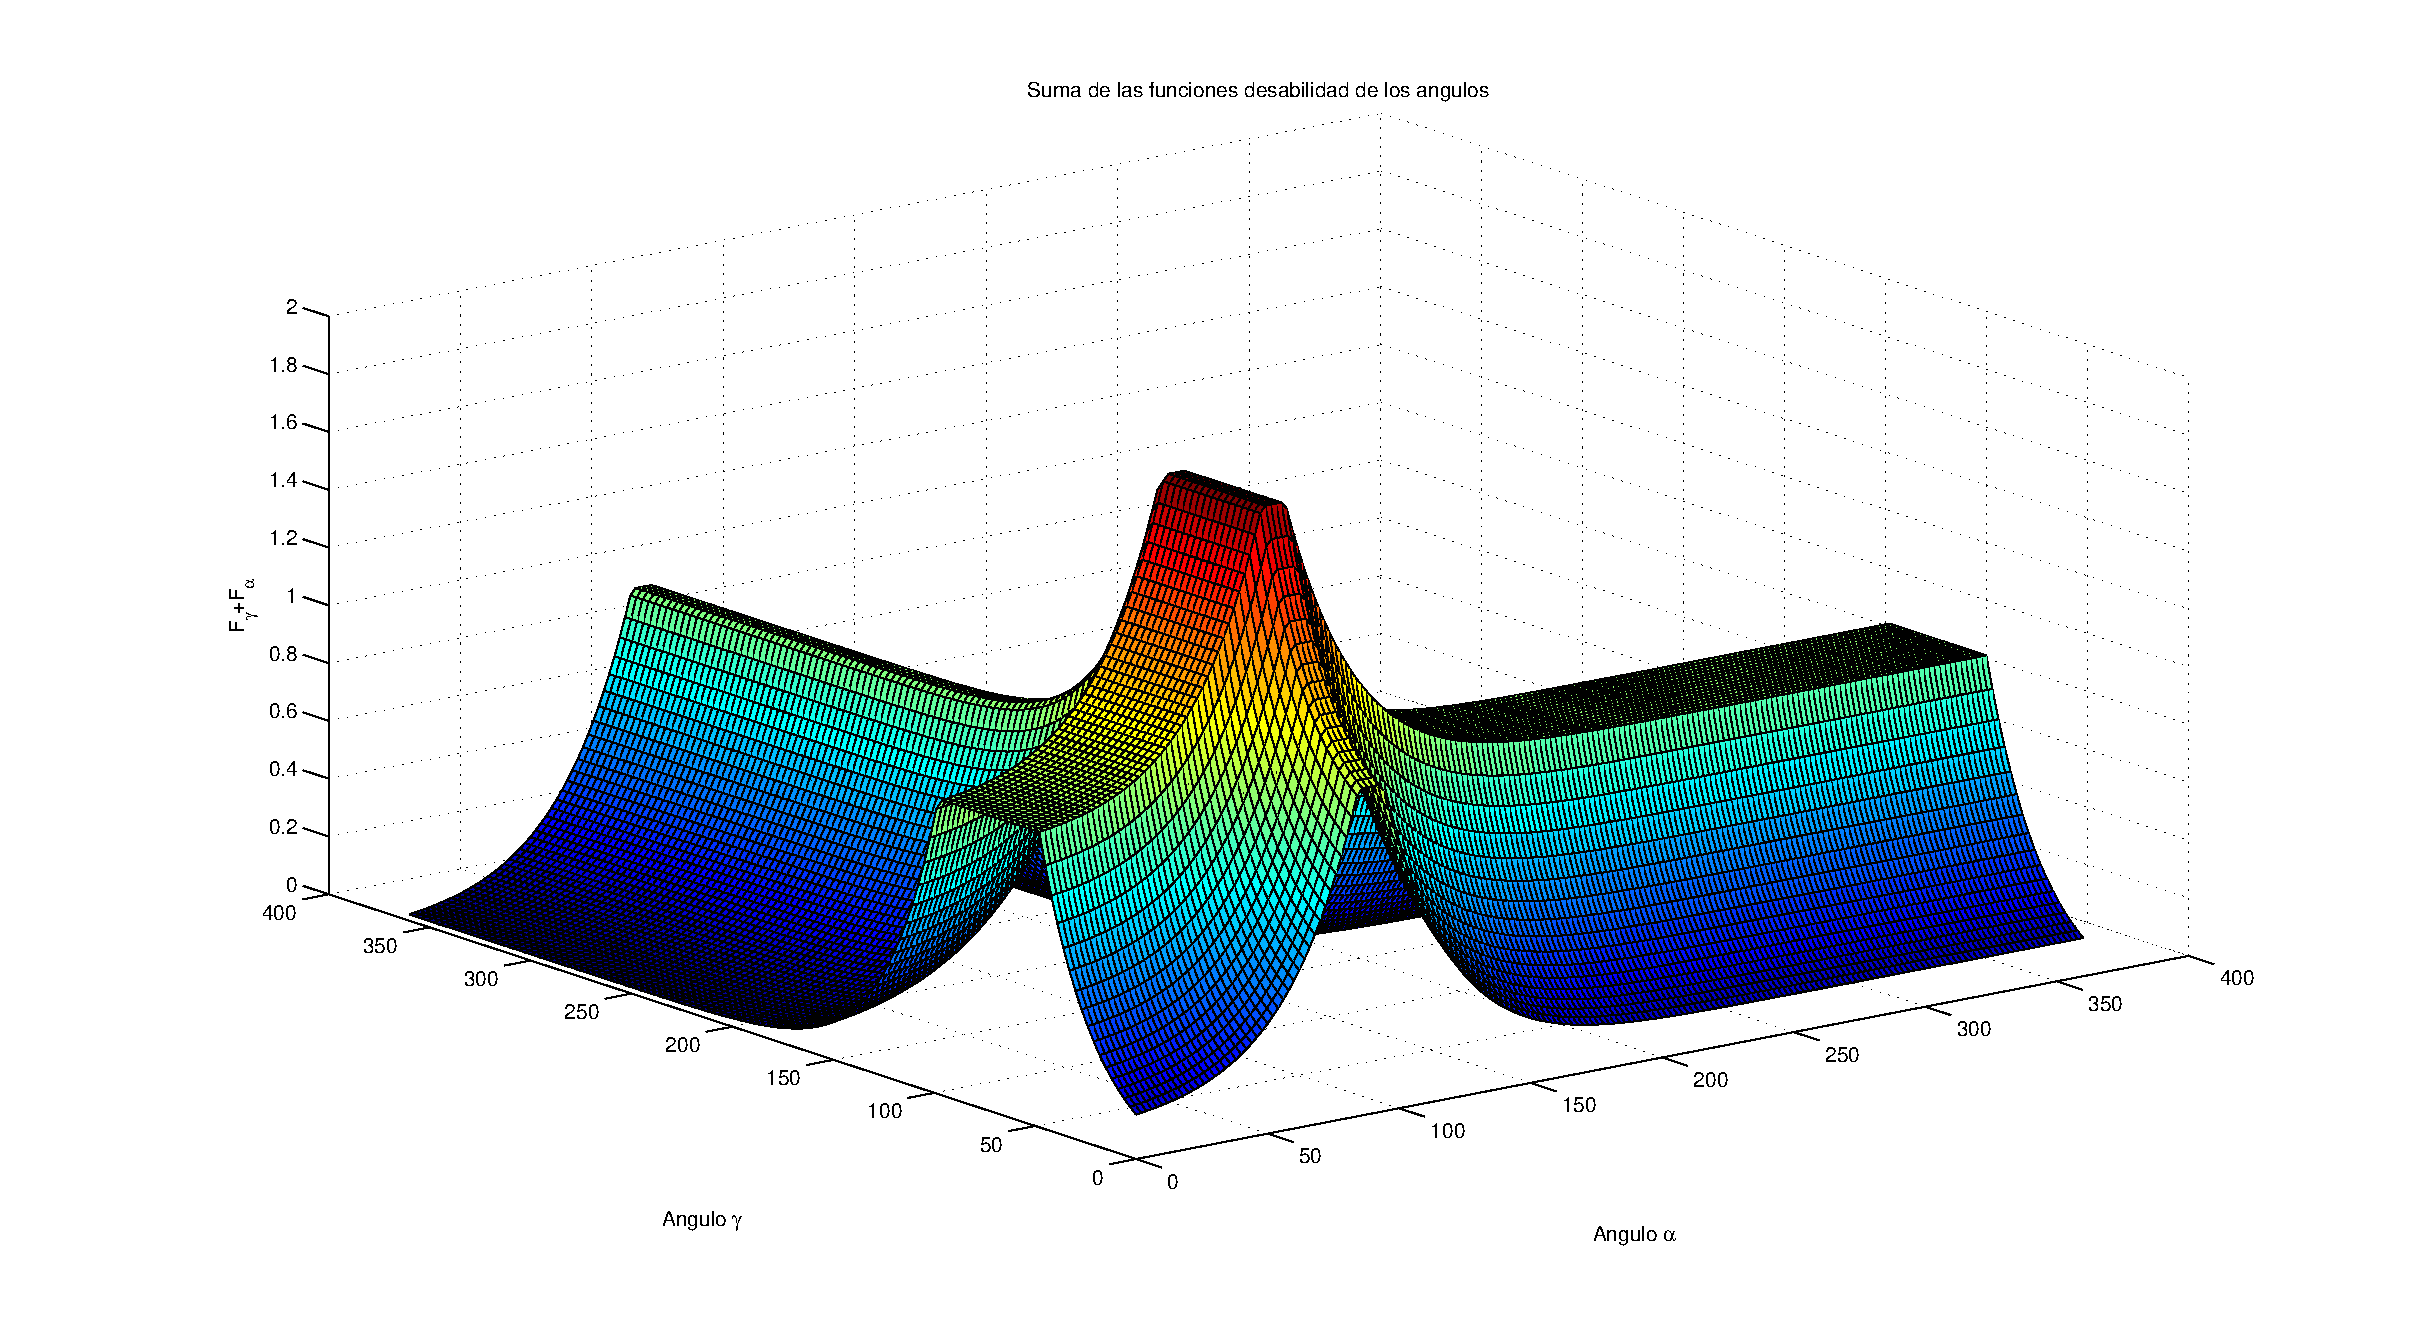
\includegraphics[height=9cm,angle=0]{fdeseabilidadsuma.eps}
\caption{Suma de las funciones deseabilidad tipo Derringer de los \'angulos 
internos del tri\'angulo unitario}
\end{figure}
%%%%%%%%%%%%%%%%%%%%%%%%%%%%%%%%%%%%%%%%%%%%%%%%%%%%%%
La suma de las funciones deseabilidad para los dos \'angulos ($d_{\alpha}$ y 
$d_{\gamma}$) calculados por el AG se muestra en la figura 3.2.
%~\ref{fig1}.


Para encontrar las matrices de masa de los quarks compatibles con los datos 
experimentales se utliza AG para optimizar la funci\'on  deseabilidad, $F_d$,
que es la suma de las doce funciones individuales
$$F_d=\sum^{12}_{i=1}d_i+d_J+d_{\alpha}+d_{\gamma},$$
y tiene un valor m\'aximo de 12, justo cuando los doce par\'ametros que se
intentan ajustar est\'an dentro del intervalo experimental.  


\newpage}

{\normalsize
\chapter{Resultados}
\index{Resultados}

Se utiliz\'o un conjunto de masas en los intervalos reportados por Koide 
~\cite{Fus199701}, Xing ~\cite{xin200801} y Emmanuel-Costa ~\cite{Emm200901} 
que pudieran ajustarse a los datos experimentales de la mezcla de los quarks y
la violaci\'on de $CP$. Primero se hizo el ajuste con matrices de masa que 
presentaran en ambos sectores la textura de Fritzsch con dos ceros dada en la
ecuaci\'on ~(\ref{matfrit}), \'este es el modelo $F4$ presentado en la tabla 
4.1.
%~\ref{ttt1}. 
 
{\tiny
\begin{table}[h!]\label{ttt1}
\begin{scriptsize}
\caption{Matrices de {masa} hermitianas de los quarks puestas a prueba}
$$\ba{c|ccccc}\hline\hline
 & F4 & F2F3 & F3F2 & F2R1 & R1F2\\ \hline \\
M_u&\left(\ba{ccc} 0&A&0\\ A*&D&B\\ 0&B&C \ea\right) & 
\left(\ba{ccc} 0&A&0\\ A*&D&B\\ 0&B*&C \ea\right) & 
\left(\ba{ccc} 0&A&O\\ A*&0&B\\ 0&B*&C \ea\right) & 
\left(\ba{ccc} 0&A&0\\ A*&D&B\\ 0&B*&C \ea\right) & 
\left(\ba{ccc} 0&A&0\\ A*&D&0\\ 0&0&C \ea\right)\\  \\ \hline\\
M_d&\left(\ba{ccc} 0&A&0\\ A*&D&B\\ 0&B*&C \ea\right) & 
\left(\ba{ccc}     0&A&0\\ A*&0&B\\ 0&B*&C \ea\right) & 
\left(\ba{ccc}     0&A&0\\ A*&D&B\\ 0&B*&C \ea\right) & 
\left(\ba{ccc}     0&A&0\\ A*&D&0\\ 0&0&C \ea\right) & 
\left(\ba{ccc}     0&A&0\\ A*&D&B\\ 0&B*&C \ea\right)\\  \\ \hline
\ea $$
\end{scriptsize}
\end{table}
}


Se utiliz\'o un AG por 2160 generaciones para cada uno de los intervalos de la
dadas en la tabla ~\ref{t3masas}. Los resultados obtenidos para los m\'odulos de
la matriz de mezcla con el valor mayor de la funci\'on deseabilidad, $F_d$,
despu\'es de todas las generaciones son presentados en la tabla 4.2. En los
primeros 10 renglones de la tabla 4.2 se presentan los m\'odulos de la matriz de
mezcla te\'oricos obtenidos para cada uno de los tres conjuntos de intervalos de
masas y el cociente de los dos primeros m\'odulos del tercer rengl\'on en la
matriz $V_{ckm}$. En la \'ultima columna se presentan los valores actuales para
los m\'odulos de la matriz de mezclas ~(\ref{pdgvckm}) y reportados en 
~\cite{Nak201001}. En el \'ultimo rengl\'on de la tabla 4.2 se observa que el 
\'unico conjunto de intervalos de masa con los que se obtuvieron resultados que
pudieron ajustarse a los datos experimentales son los reportados por Koide
~\cite{Fus199701}, es decir, la funci\'on deseabilidad tom\'o su valor m\'aximo,
lo que significa que todos los observables ajustados est\'an dentro del error
experimental y a los cuales les corresponde una $\chi^2=0.35$ calculada de la
manera reportada en PDG ~\cite{Nak201001}. Los par\'ametros que se utilizaron
para hacer el ajuste son las seis masas de los quarks y cinco par\'ametros
libres, de los cuales tres son fases. El ajuste con las masas reportadas por
Emmanuel-Costa tiene un valor de la funci\'on deseablidad mayor al obtenido con
las masas reportadas por Xing y un valor de $\chi^2$ menor. Sin embargo, ambos
ajustes son malos, ya que la funci\'on deseabilidad es menor a 12, y por lo
tanto, no todos los observables pudieron ser ajustados simult\'aneamente para un
mismo conjunto de par\'ametros.

{\tiny
\begin{table}[h!]\label{tra}
\caption{Valores te\'oricos obtenidos de $|V_{ij}|$ utilizando la texturas con 
cuatro ceros de Fritzsch (F4) para las matrices de masa presentadas en la tabla 
~\ref{t3masas} y los valores experimentales de $|V_{ij}|$.}
$$\ba{l|ccc|r}
|V_{ckm}|^{teo} & \mbox{Koide} & \mbox{Emmanuel-Costa} & \mbox{Xing} & 
|V_{ckm}|^{exp}\\ \hline
|V_{ud}| & 0.97426 & 0.97412 & 0.97414 & 
0.97428\pm{0.00015} \\
|V_{us}| & 0.22537 & 0.22599 & 0.22589 & 
0.2253\pm{0.0007} \\
|V_{ub}| & 0.00343 & 0.00335 & 0.00187 & 
0.00347^{+0.00016}_{-0.00012} \\
|V_{cd}| & 0.22523 & 0.22588 & 0.22589 & 
0.2252\pm{0.0007} \\
|V_{cs}| & 0.97345 & 0.97343 & 0.97409 & 
0.97345^{-0.00015}_{-0.00016} \\
|V_{cb}| & 0.04082 & 0.03748 & 0.01090 & 
0.0410^{+0.0011}_{-0.0007} \\
|V_{td}| & 0.00869 & 0.00813 & 0.00184 & 
0.00862^{+0.00026}_{-0.00020} \\
|V_{ts}| & 0.04003 & 0.03674 & 0.01091 & 
0.0403^{+0.0011}_{-0.0007} \\
|V_{tb}| & 0.999160 & 0.999291 & 0.999939 & 
0.999152^{+0.000030}_{-0.000045} \\
|V_{td}|/|V_{ts}| & 0.2171 & 0.2213 & 0.1685 & 0.21\pm{0.04} \\
\chi^2& 0.350 & 40.456 &2752 \\
F_d & 12 & 11.938 & 11.381 & 12 \\
\ea
$$\end{table} }
  
En la tabla 4.3 se muestran los valores ajustados para los observables de
la violaci\'on de $CP$, solo los datos de la primera columna est\'an en el
intervalo de error reportado experimentalmente. En la ecuaci\'on ~(\ref{supuni})
del cap\'itulo anterior se presenta la forma de la matriz $V_{ckm}$ te\'orica
la cual es unitaria. La suma de dos \'angulos internos de los tri\'angulo
unitario se determina el valor del tercero. Los valores presentados
en la tabla 4.3 de los \'angulos $\alpha$ y $\gamma$ se obtuvieron a 
partir de las ecuaciones ~(\ref{alpha}) y ~(\ref{gamma}), el valor del \'angulo
$\beta$ de la condici\'on de unitariedad, con lo que se asegura la existencia
del tri\'angulo unitario y que la suma de los tres \'angulos deber ser 180. Por
\'ultimon el valor te\'orico reportado para el invariante de Jarlskog se
calcul\'o de la ecuaci\'on ~(\ref{idj}).
 
{\tiny
\begin{table}[h!]\label{tra2}
\caption{Valores te\'oricos obtenidos de $\alpha$, $\beta$, $\gamma$ y $J$ para 
las texturas con cuatro ceros de Fritzsch (F4) para las matrices de masa presentadas en la tabla ~\ref{t3masas} y los valores experimentales.}
$$\ba{l|ccc|r}
 & \mbox{Koide} & \mbox{Emmanuel-Costa} & \mbox{Xing} &\mbox{exp}\\ \hline
\alpha & 87.9 & 84.6 & 84.6 & 89.0^{+4.4}_{-4.2}  \\
\gamma & 70.7 & 72.8 & 48.0 & 73^{+22}_{-25}      \\
\beta  & 21.3 & 22.6 & 47.4 & 21.1495^{+0.905}_{-0.8787} \\
J (10^{-5})& 2.901 & 2.64 & 0.333 & 
2.91^{+0.19}_{-0.11} \\
\ea
$$\end{table} }

Los par\'ametros de entrada con los que se obtuvieron los valores reportados
en las tablas 4.2 y 4.3 se presentan en la tabla 4.4. Los intervalos de las
masas son los presentados en la tabla ~\ref{t3masas} y los intervalos para los
par\'ametros $D_q$ son escogidos de tal manera que los elementos de la matriz
sim\'etrica $\tilde M_q$ de la ecuaci\'on ~(\ref{matsim}) sean reales. Los
valores de las fases en los \'ultimos tres renglones son libres y sin relaci\'on
alguna, sus intervalos son de $0\leq f_i\leq 360$. En la tabla 4.4, enter todas
las soluciones en las que se obtuvo un valor de la funci\'on deseabilidad de
doce, utilizando las masas de Koide, se presenta el conjunto al que le
corresponde un valor menor de $\chi^2$. En las otras dos columnas se presentan
los conjuntos de valores para los par\'ametros de entrada con los que se obtuvo
el mayor valor de la funci\'on deseabilidad.

{\tiny
\begin{table}[h!]\label{trare}
\caption{Valores de los par\'ametros con los que se obtienen los resultados de
los ajustes n\'umericos presentados en las tablas 4.2 y 4.3.}
$$\ba{l|ccc}
 & \mbox{Koide} & \mbox{Emmanuel-Costa} & \mbox{Xing} \\ \hline
m_u & 0.00274 & 0.00199 & 0.00176 \\
m_c & 0.61606 & 0.55000 & 0.66717 \\
m_t & 169.567 & 170.661 & 169.954 \\
D_u & 159.783 & 164.387 & 106.365 \\
m_d & 0.00403 & 0.00210 & 0.00485 \\
m_s & 0.10409 & 0.07499 & 0.10495 \\
m_b & 2.97899 & 2.87811 & 2.80000 \\
D_d & 2.80023 & 2.76944 & 1.72287 \\
f_1 & 75.60   & 135.71  & 10.79   \\
f_2 & 74.97   & 135.74  & 104.53  \\
f_3 & 75.77   & 136.73  & 104.73  \\
\ea
$$\end{table} }

Dado que con las masas de Koide se pudieron ajustar simult\'aneamente los
m\'odulos de la matriz de mezcla y los par\'ametros de la violaci\'on de $CP$
te\'oricos a los datos experimentales cuando las matrices de masa presentan
texturas de Fritzsch con dos ceros en ambos sectores (F4), se usan estos
intervalos de masa para intentar obtener resultados que se ajusten a los datos
experimentales utilizando texturas diferentes. Los modelos que se usaron para
las matrices de masa fueron las texturas de Fritzsch con cinco ceros (F2F3 y
F3F2) y la textura de Fritzsch con cuatro ceros (F4), y las texturas I y IV de
Ramond, las cuales son presentadas en la tabla 4.1. Los cinco resultados se
obtuvieron utilizando algoritmos gen\'eticos durante 2160 generaciones. 

{\tiny
\begin{table}[h!]\label{trbb}
\caption{Valores te\'oricos obtenidos de $|V_{ij}|$ utilizando las texturas 
presentadas en la tabla 4.1  para las matrices de masa de Koide presentadas en 
la tabla ~\ref{t3masas}.}
$$\ba{l|ccccc|r}
|V_{ckm}|^{teo} & \mbox{F4-90} & \mbox{F2F3} & \mbox{F3F2 (II)} & 
\mbox{F2R1 (IV)} & \mbox{R1F2 (I)} & 
|V_{ckm}|^{exp}\\ \hline
|V_{ud}| & 0.97415 & 0.97415 & 0.97047 & 0.97263 & 0.96233 & 
0.97428\pm{0.00015} \\
|V_{us}| & 0.22591 & 0.22590 & 0.22460 & 0.22550 & 0.22460 & 
0.2253\pm{0.0007} \\
|V_{ub}| & 0.00055 & 0.00026 & 0.08803 & 0.05601 & 0.15320 & 
0.00347^{+0.00016}_{-0.00012} \\
|V_{cd}| & 0.22590 & 0.22590 & 0.22569 & 0.22590 & 0.22773 & 
0.2252\pm{0.0007} \\
|V_{cs}| & 0.97409 & 0.97415 & 0.97418 & 0.97414 & 0.97366 & 
0.97345^{-0.00015}_{-0.00016} \\
|V_{cb}| & 0.01083 & 0.00151 & 0.00594 & 0.00375 & 0.01072 & 
0.0410^{+0.0011}_{-0.0007} \\
|V_{td}| & 0.00244 & 0.00026 & 0.08521 & 0.05437 & 0.14849 & 
0.00862^{+0.00026}_{-0.00020} \\
|V_{ts}| & 0.01056 & 0.00152 & 0.02291 & 0.01395 & 0.03915 & 
0.0403^{+0.0011}_{-0.0007} \\
|V_{tb}| & 0.999941 & 0.999999 & 0.996100 & 0.998423 & 0.988138 & 
0.999152^{+0.000030}_{-0.000045} \\
|V_{td}|/|V_{ts}| & 0.2307 & 0.1685 & 3.7184 & 3.8969 & 3.7925 & 0.21\pm{0.04} \\
\chi^2& 2922.87 & 4579.7  & 374586  & 141387  & 1260082 \\
F_d   & 11.662  & 11.567  & 10.046  & 10.310  & 9.583   & 12 \\
\ea
$$\end{table} }
Se observa en el \'ultimo rengl\'on de la tabla 4.4 que con ninguna textura se
pudo obtener resultados que se ajusten satisfactoriamente a los datos
experimentales. En la primera columna se presentan los resulatados de imponer
que la fase $f_1$ sea de 90 grados y las otras dos fases tomen un valor de cero
usando el modelo de 4 ceros de Fritzsch la funci\'on deseabilidad no alcanz\'o
su valor m\'aximo, por esto el ajuste es malo. Al resto de las texturas se les
permiti\'o como par\'ametro libre la matriz de fases y no ajustaron los datos
experimentales, teniendo un mejor resultado aquellas donde la matriz de masa del
sector $u$ presenta la textura de dos ceros de Fritzsch, y de ellas la textura
de cinco ceros de Fritzsch (F2F3) ajusta mejor (la funci\'on deseabilidad es
mayor y el valor de $\chi^2$ menor) que la cuarta textura de Ramond (F2R1). 

En la tabla 4.6 se presentan los valores de los par\'ametros de la
violaci\'on de $CP$ correspondientes a las matrices de mezcla con las que se
obtuvo la tabla 4.5 y fueron calculados de la misma manera antes
explicada.

{\tiny
\begin{table}[h!]\label{trba}
\caption{Valores te\'oricos ajustados de los observables $\alpha$, $\beta$,  
$\gamma$ y $J$ para las cinco texturas presentadas en la tabla 4.1
utlilizando las masas de Koide.}
$$\ba{l|ccccc|r}
 &\mbox{F4-90}&\mbox{F2F3}&\mbox{F3F2 (II)}&\mbox{F2R1 (IV)}&\mbox{R1F2 (I)}&
\mbox{exp}\\ \hline

\alpha & 84.6 & 84.6 & 0.82 & 0.87 & 0.91 & 89.0^{+4.4}_{-4.2}  \\
\gamma & 82.7 & 48.0 & 64.9 & 76.7 & 73.1 & 73^{+22}_{-25}      \\
\beta  & 12.6 & 47.4 & 114.2 & 102.4 & 106.0 & 21.1495^{+0.905}_{-0.8787} \\
J (10^{-5})& 0.006   & 10.38 & 30.73 & 4.478 & 34.446 & 
2.91^{+0.19}_{-0.11} \\
\ea
$$\end{table} }


Los par\'ametros de entrada con los que se obtuvieron los valores reportados
en las tablas 4.5 y 4.6 se presentan en la tabla 4.7.
Los valores de las fases en los \'ultimos tres renglones  de la primera columna
(F4-90) corresponden a las restricciones impuestas al espacio de los
par\'ametros de entrada. El valor de cero para $D_d$ y $D_u$ en la segunda
(F2F3) y tercera (F3F2) columna respectivamente corresponden a las restricciones
propias de ambos modelos de texturas. El valor de cero para $D_d$ y $D_u$ en la
tercera (F3F2) y cuarta (F2R1) columna respectivamente corresponden a los
valores encontrados por el AG\footnote{Los par\'ametros en los que aparece * no
son libres, y est\'an determinados a partir de las masas de los quarks.}. En la
\'ultima columna se presentan los intervalos de masa reportados por Koide.

{\tiny
\begin{table}[h!]\label{trare2}
\caption{Valores de los par\'ametros con los que se obtienen los resultados de
los ajustes n\'umericos presentados en las tablas 4.5 y 4.6} 
%~\ref{trb2} y ~\ref{trba}}
$$\ba{l|ccccc|c}
 &\mbox{F4-90}&\mbox{F2F3}&\mbox{F3F2 (II)}&\mbox{F2R1 (IV)}&\mbox{R1F2 (I)}
&\mbox{masa de Koide} \\ \hline
m_u   & 0.00188 & 0.00193 & 0.00275 & 0.00275 & 0.00275 & 
0.00233^{+0.00045}_{-0.00042}\\
m_c   & 0.73296 & 0.61834 & 0.73299 & 0.61600 & 0.61600 & 
0.677^{+0.056}_{-0.61}\\
m_t   & 173.461 & 178.497 & 168.000 & 193.999 & 168.408 & 
181\pm13\\
D_u   & 109.954 &   5.315 & 0.0     & 0.00000 & *       & \\
m_d   & 0.00503 & 0.00528 & 0.00529 & 0.00529 & 0.00529 & 
0.00469^{+0.0060}_{-0.0066}\\
m_s   & 0.10519 & 0.10499 & 0.08040 & 0.08040 & 0.08040 & 
0.0934^{+0.0118}_{-0.0130}\\
m_b   & 2.89000 & 2.89000 & 3.10999 & 2.89000 & 3.11000 & 
3\pm0.11\\
D_d   & 1.79936 & 0.0     & 0.00000 & *       & 0.00000 & \\
f_1   & 90.0    & 269.94  & 1.47    & 205.87  & 98.2    & \\
f_2   &  0.0    & 0.001   & 62.69   & 268.73  & 162.5   & \\
f_3   &  0.0    & 0.076   & 62.93   & 0.00    & 0.00    & \\
\ea
$$\end{table} }


Como se sabe en la naturaleza solo hay una fase responsable de la violaci\'on de
$CP$, adem\'as los observables de la matriz de mezcla de los quarks son 
invariantes ante el refasamiento de los quarks. En el ajuste num\'erico 
presentado en la tabla 4.4 se ve claramente que en los tres casos dos 
fases son iguales entre s\'i, por lo que se puede absorber una fase en los 
campos de los quarks qued\'andose con una sola fase responsable de la 
violaci\'on de $CP$ en el modelo. Por esta raz\'on se hizo un ajuste num\'erico 
con las masas de Koide haciendo que una fase sea igual a cero, $f_2=0$, y las
otras dos fases sean iguales entre s\'i, $f_1=f_3$, pero variando libremente.
Para lo anterior se us\'o la textura con cuatro ceros de Fritzsch (F4) y
las matrices de masa que se obtienen de este ajuste son las siguientes, 
\be
M_u=\left(\ba{ccc} 0&0.16877&0\\
0.16877&171.67256&44.34728\\
0&44.34728&10.80211\ea\right),
\ee
donde la matriz de masa para los quarks $u$ es real y toda la violaci\'on de 
$CP$ viene de la matriz de masa compleja del sector $d$ 
\be
M_d=\left(\ba{ccc} 0&0.12462e^{-0.80017i}&0\\
0.12462e^{0.80017i}&2.75342&0.72220e^{0.80017i}\\
0&0.72220e^{-0.80017i}&0.08719\ea\right).
\ee
Con estas matrices de masa la func\'on deseabilidad toma su valor m\'aximo, 
$F_d=12$, por lo tanto todos los observable se ajustan simult\'aneamente a los
datos experimentales.


\newpage}

{\normalsize
\chapter{Conclusiones}

Las texturas de Fritzsch con 2 ceros en ambos sectores permiten un excelente 
ajuste ($F_d=12$ y $\chi^2=0.350$) a los datos experimentales, utilizando los
 valores de los intervalos de masas para los quarks reportados por Koide. Los 
nueve m\'odulos de los elementos de la matriz de mezclas, los tres \'angulos del
tri\'angulo unitario y el invariante de Jarlskog obtenidos est\'an de acuerdo 
con los valores centrales reportados ~\cite{Nak201001}. Las texturas no permiten
hacer predicciones para la matriz de mezclas ya que se tienen m\'as de cuatro 
par\'ametros en la matriz de mezcla te\'orica.

El ajuste num\'erico sugiere que los tres pares de texturas de Robert 
~\cite{rrr} estudiadas en el presente trabajo (F3F2, F2R1 y R1F2) son reducidas 
de texturas con cinco ceros a texturas con seis ceros, en donde el par\'ametro 
libre $D_q$ es ajustado en la optimizaci\'on a cero. 

Con el conjunto de masas de los quarks reportado por Koide, la textura con
cuatro ceros (F4) en las matrices de masa y las restricciones en el espacio de
los par\'ametros de las fases no se consigui\'o un resultado \'optimo, ya que la
funci\'on deseabilidad $F_d=11.662$ no es 12 y la $\chi^2=2922.9$ es muy grande.
Para la textura F4 no se pudo encontrar un resultado compatible con el maximal
en el invariante de Jarlskog.

A partir de los datos presentados en la tabla 4.2 se concluye que no se 
pudo ajustar a los datos experimentales de la mezcla de los quarks y 
violaci\'on de $CP$ con las masas reportadas por Xing y Emmanuel-Costa 
utilizando texturas de Fritzsch con dos ceros en ambos sectores. 

A partir de las masas de Koide no se pudo obtener que la matriz de mezcla, los
\'angulos del tri\'angulo unitario y el invariante de Jarlskog ajustaran de
manera simult\'anea con los otros cuatro pares de texturas de cinco ceros
estudiados.

La optimizaci\'on con AG no es un m\'etodo exhaustivo por lo tanto no se puede
asegurar que los modelos en los que no se pudo obtener el valor m\'aximo de la
funci\'on deseabilidad no sean compatibles con los datos experimentales. 
Es posible que si las funciones
deseabilidad individuales sean iguales a la propuesta por Derringer, y en lugar
de que la funci\'on deseabilidad sea la suma de las doce funciones individuales
sea la media geom\'etrica, se obtengan mejores resultados. Otra posible mejora
es que la selecci\'on no sea elitista, ya que esta elecci\'on pudo crear 
c\'omulos grandes de soluciones optimizando un m\'inimo local.

Una propuesta para darle continuidad a este trabajo es agregar hip\'otesis de
nueva f\'isica, como la presntada en el cap\'itulo 3 \cite{Bra200601}, a los
modelos con los que no se puedan obtener resultados que
se ajusten a los datos experimentales, con la intenci\'on de investigar si con
ellas si es posible. Otra propuesta est\'a dirigida a la mejora del
m\'etodo. Por ejemplo, adem\'as de comparar la eficiencia del AG actual contra
aqu\'el donde se apliquen las propuestas del p\'arrafo anterior, se podr\'ian
obtener los intervalos en los par\'ametros de entrada para los cuales la
funci\'on deseabilidad sea 12.

\newpage}

\appendix
{\normalsize
\chapter{Mecanismo de Higgs}
Cuando existe rompimiento de simetr\'ia el resultado es un campo 
vectorial con masa, junto con el campo escalar del Higgs que tambi\'en tiene 
masa. Que un generador $\mathcal{G}$ deje invariante el vac\'io significa que 
$$
e^{i\alpha \mathcal{G}}\langle\Phi \rangle_0=\langle\Phi\rangle_0.
$$
Para una transformaci\'on infinitesimal lo anterior se  expresa como
$$
(1+i\alpha \mathcal{G})\langle\Phi\rangle_0=\langle\Phi\rangle_0,
$$
as\'i que la condici\'on para que $\mathcal{G}$ deje invariante el vac\'io es 
$$
\mathcal{G}\langle\Phi\rangle_0=0.
$$
Si los generadores de $\gme$ rompen la simetr\'ia local, los bosones de norma
correspondientes adquirir\'an masa. Se busca que s\'olo uno de ellos, el 
fot\'on, permanezca sin masa. Para los generadores de $\gme$ se tienen los 
siguientes c\'alculos
\be\label{6.3.23}
\tau_1\vevh=\mpi\left(\ba{c} 0\\ v \ea\right)=\left(\ba{c} v\\ 0 \ea\right)
\neq 0,
\ee
\be\label{6.3.24}
\tau_2\vevh=\mpii\left(\ba{c} 0\\ v \ea\right)=\left(\ba{c} -iv\\ 0 \ea\right)
\neq 0,
\ee
\be\label{6.3.25}
\tau_3\vevh=\mpiii\left(\ba{c} 0\\ v \ea\right)=\left(\ba{c} 0\\ -v \ea\right)
\neq 0,
\ee
\be\label{6.3.26}
Y\vevh=+1\vevh\neq 0,
\ee
con lo que se ve que hay rompimiento de simetr\'ia. Utilizando la relaci\'on de
Gell-Mann-Nishijima ~(\ref{rgmn}) se observa que
\be\label{27}
Q\vevh=\frac{1}{2}\left(\tau_3+\frac{Y}{2}\right)\vevh=0.
\ee
Los cuatro generadores rompen la simetr\'ia ~(\ref{6.3.23}-\ref{6.3.26}), pero 
la combinaci\'on lineal correspondiente a la carga el\'ectrica ~(\ref{rgmn}) 
deja invariante el vacio ~(\ref{27}), as\'i el fot\'on permanecer\'a sin masa
\footnote{Para mayor detalle en la lagrangiana de Higgs ver ap\'endice 1} 

En la lagrangiana de Higgs ~(\ref{lhiggs}) la energ\'ia potencial
$V(\Phi^{\dag}\Phi)$ tiene la forma
$$
V(\Phi^{\dag}\Phi)=\frac{m^2}{2v^2}[(\Phi^{\dag}\Phi)-v^2]^2.
$$
Cuando se sustituye el valor del estado excitado ~(\ref{vevhe}) se obtiene el
potencial del Higgs despu\'es del rompimiento espont\'aneo de simetr\'ia, cuya
expresi\'on es
\be\label{phdres}
V(\Phi^{\dag}\Phi)=m^2h^2+\frac{m^2h^3}{\sqrt{2}v}+\frac{m^2h^4}{8v^2}=V(h),
\ee
con lo cual la densidad lagrangiana invariante de norma localmente para el 
Higgs es
$$
\mathcal{L}_{\Phi}=(D_{\mu}\Phi)^{\dag}(D^{\mu}\Phi)-V(h)
$$
donde $D_{\mu}$ es la derivada covariante dada por ~(\ref{dcme}). Entonces, 
usando ~(\ref{vevhe}) la lagrangiana toma la forma
$$\ba{lr}
\mathcal{L}_{\Phi}&=\frac{1}{2}\partial_{\mu}h\partial^{\mu}h+\frac{g^2_2}{4}
\left(W^1_{\mu}+iW^2_{\mu}\right)\left(W^{1\mu}-iW^{2\mu}\right)\left(v+
\frac{h}{\sqrt{2}}\right)^2\\ &+\left[\frac{g^2_2}{4}W^3_{\mu}W^{3\mu}-
\frac{g_1g_2}{2}W^3_{\mu}B^{\mu}+\frac{g^2_1}{4}B_{\mu}B^{\mu}\right]\left(v+
\frac{h}{\sqrt{2}}\right)^2-V(h)\ea
$$

que se reduce a

\be\label{lh}
\mathcal{L}_{\Phi}=\frac{1}{2}\partial_{\mu}h\partial^{\mu}h+\frac{g^2_2}{2}
W^-_{\mu}W^{+\mu}\left(v+\frac{h}{\sqrt{2}}\right)^2+\frac{1}{4}\left(g^2_2
+g^2_1\right)Z_{\mu}Z^{\mu}\left(v+\frac{h}{\sqrt{2}}\right)^2-V(h).
\ee
Los t\'erminos en ~(\ref{lh}) proporcionales al cuadrado de $v$ son t\'erminos 
de masa. Los campos de los bosones $W^{1\mu}$ y $W^{2\mu}$ fueron reemplazados 
por la combinaci\'on lineal de ellos
\be\label{cnws}
W^{\pm}\equiv\frac{(W^{\mu}_1\mp iW^{\mu}_2)}{\sqrt{2}}.
\ee
La  forma de $Z^{\mu}$ es
\be\label{bz}
Z^{\mu}=W^{3\mu}\cos\theta_W-B^{\mu}\sin\theta_W,
\ee
donde
$$
\cos\theta_W=\frac{g_2}{\left(g^2_1+g^2_2\right)^{\frac{1}{2}}},\qquad
\sin\theta_W=\frac{g_1}{\left(g^2_1+g^2_2\right)^{\frac{1}{2}}}.
$$
A $\theta_W$ se le llama el \'angulo de Weinberg. Se observa en ~(\ref{lh}) que
despu\'es del rompimiento de simetr\'ia los bosones de norma $W^{\pm\mu}$ y 
$Z^{\mu}$ adquieren masa.




\newpage}

{\normalsize
\chapter{C\'odigo}
C\'odigo en Matlab 8 ~\cite{matlab} de la funci\'on que se usa para poner a
prueba los modelos de texturas utilizando algoritmos gen\'eticos y las funciones
que se usan en ella.
\section{Algoritmo Gen\'etico}
\begin{verbatim}
%% Algoritmo Genetico
% Proporciona los valores de las masas, fases y parametros libres que mejor
% ajusten a los valores experimentales a los modelos de las texturas en las
% matrices de masa.
%Los parametros de entrada son n= el tamano de la poblacion.
%bmasas=intervalos de masas que se usan 1=Xing, 2=Koide y 3=Emmanuel-Costa
%bpdg  =datos experimenteles con los que se compararan los modelos,
%dependiendo del ano 
%bt = al modelos de la textura puesto a prueba 1=F4, 2=F2F3, 3=F3F2, 4=F2R1 
% y 5=R1F2.

function [poblacion,hist] = funalg_texturas_ultimate3(n,bmasa,bpdg,bt)

%% Parametros iniciales
% Se configua el Algoritmo definiendo parametros analogos en la Genatica
format long
 %Se crean la poblacion inicial y se cargan los datos experimentales.
%[poblacion,imu,imd,V,Vint,Ver,angu]=fundatexp(n,bmasa,bpdg);     
                             
generaciones = 15;            %Numero de generaciones que se dejara evolucionar
                              %al sistema
guardar      = 3;             %Numero de datos que se guardan
nC           = 20;            %Numero de cuates por parejas
migra        = 0;             %Generacion espontanea  
probabilidad = 1.0;           % probabilidad de que cada gen mute
hist=ones(guardar,12);        %Se crea la matriz hist. Donde se guada la 
                              %evolucion de la poblacion
par=11;                       %Parametros
obs=1;                        %Observables
                              %Maximo valor de la mutacion
mutacion = [0.00000250 0.0003 0.0115 0.00250 0.00000350 0.00075 0.00035 0.00250
            0.01 0.01 0.01]/5;
%% Poblaci�n inicial
% Se genera aleatoriamente una poblacion inicial de posibles soluciones.
% Las primeras 4 columnas representan los genes del sector u. Las
% siguientes 4 columnas representan los genes del sector d. Las ultimas 4
% columnas son las 3 fases posibles y la funcion desebilidad.
% Cada uno de los n individuos (renglones) representa una posible soluci�n.
%poblacion = rand(n,2);
imu=zeros(2,4);
imd=zeros(2,7);
[poblacion,imu,imd,V,Vint,Ver,ang]=fundatexp(n,bmasa,bpdg);

%% Iteraciones
% La poblacion de soluciones evoluciona mediante la cruza y mutacion
for ci= 1:guardar
    hw = waitbar(0,'Evolucionando...');
    for i = 1:generaciones
        temporal=zeros(2*(n*(nC+1)+migra),par+obs);
        %% Orden aleatorio de parejas
        % La formacion de parejas para la reproduccion es aletoria
        poblacion(:,par+1:obs+par) = rand(n,obs);
        poblacion = sortrows(poblacion,+(par+1));
        temporal(1:n,:) = poblacion;
%% Cruza
        for j=1:n/2
            mama=rand(nC,par+obs)>0.5;
            papa=~mama;
            temporal(n+1+   (2*nC*(j-1)):n+   (2*nC*(j-1))+nC,:) =
repmat(poblacion(2*j,:),nC,1).*mama + repmat(poblacion(2*j-1,:),nC,1).*papa;
            temporal(n+1+nC+(2*nC*(j-1)):n+nC+(2*nC*(j-1))+nC,:) =
repmat(poblacion(2*j,:),nC,1).*papa + repmat(poblacion(2*j-1,:),nC,1).*mama;
        end
 %Generacion Espontanea
        temporal(n*(nC+1)+1:n*(nC+1)+migra,:) = [repmat(imu(1,:),migra,1)+
repmat((imu(2,:)-imu(1,:)),migra,1).*rand(migra,4) repmat(imd(1,:),migra,1)+
repmat((imd(2,:)-imd(1,:)),migra,1).*rand(migra,7) rand(migra,obs)];
        s=n*(nC+1)+migra;
%% Mutacion
        %Se calcula la mutacion, los limites permitidos y se muta. 
        muta=(rand(s,par+obs)*2-1).*repmat([mutacion zeros(1,obs)],s,1);
        mayor=[repmat(imu(2,:),s,1)-temporal(1:s,1:4) repmat(imd(2,:),s,1)-
temporal(1:s,5:11) zeros(s,obs)];
        menor=[repmat(imu(1,:),s,1)-temporal(1:s,1:4) repmat(imd(1,:),s,1)-
temporal(1:s,5:11) ones(s,obs)];
        b=(rand(s,par+obs)<probabilidad).*(mayor>muta).*(menor<muta);
        temporal(s+1:2*s,:)=temporal(1:s,:)+b.*muta;
%% Calculo de la aptitud (o viabilidad)
        % La columna numero 12 de poblacion representa la aptitud (viabilidad) 
        % de la solucion, mayor es mejor.
        temporal=funaptult(temporal,V,Vint,ang,bt);
        temporald = unique(temporal,'rows');
        temporalb = sortrows(temporald,-12);
        s = min([size(temporalb,1),n]);
 %Seleccion
        poblacion = temporalb(1:s,:);
        waitbar(i/generaciones,hw)
    end
    close(hw)
    hist(ci,:)=poblacion(1,:);
end

\end{verbatim}


\section{Datos experimentales}
\begin{verbatim}
%% Datos experimentales
%Proporciona los valores experimentales de los observables (los modulos de 
%la matriz de mezcla y la fenomenologia de la violacion de CP) ademas de
%losintervalos permitidos para las masas, reportados por Xing, Koide y
%Emmanule-Costa. 
%Los parametros de entrada son
%n= El tamano de la poblacion.
%bmasa= Los intervalos de masa desados 1 Xing, 2 Koide y 3. Emmanuel-Costa
%bpdg = Los valores reportados en PDG dependiendo del a\~no 1=2008 y
%2=2010.
%Los valores de salida son poblacion=poblacion inicial.
%imu=Intervalos permitidos para los qurks del sector u.
%imd=Intervalos permitidos para los qurks del sector d.
%Los valores de experimentales centrales de los modulos de la matriz Vckm.
%Los intervalos experimentales de los modulos de la matriz Vckm.
%Los valores experimentales de los observables de la violacion de CP.

function [poblacion,imu,imd,V,Vint,Ver,ang]=fundatexp(n,bmasa,bpdg)

imu=zeros(2,4);
imd=zeros(2,7);
if bmasa == 1
%%%%%%%%%%%%%%%%%%%%%%%%%%%%%%%%%%%%%%%%%%%%%%%%%%%%%%%%%%%%%%%%%%%%%%%%%%%
%%%%%%%%%%%%%%%%%%%%%%%%%%%%% Xing 2008 %%%%%%%%%%%%%%%%%%%%%%%%%%%%%%%%%%%
  imu(:,1)=0.00127+[-0.00042;0.00050];       %masa del quark u 1.4+0.6-0.5
  imd(:,1)=0.00290+[-.00119;0.001240];       %masa del quark d 2.8+-0.7
  imd(:,2)=0.055+[-0.0150;0.016];         %masa del quark s 60+15-19
  imu(:,2)=0.619+[-0.084;0.084];          %masa del quark c 0.64+0.07-0.09
  imd(:,3)=2.89+[-0.09;0.09];          %masa del quark b 2.84+0.17-0.08
  imu(:,3)=171.7+[-3;3];        %masa del quark t 170.1+-2.3
end
if bmasa == 2
%%%%%%%%%%%%%%%%%%%%%%%%%%%%%%%%%%%%%%%%%%%%%%%%%%%%%%%%%%%%%%%%%%%%%%%%%%%
%%%%%%%%%%%%%%%%%%%%%%%%%% Koide 2010 %%%%%%%%%%%%%%%%%%%%%%%%%%%%%%%%%%%%% 
 imu(:,1)=0.00233 +[-0.00045;0.00042];       %masa del quark u 1.4+0.6-0.5
 imd(:,1)=0.00469 +[-0.00066;0.00060];       %masa del quark d 2.8+-0.7
 imd(:,2)=0.0934  +[-0.0130;0.0118];         %masa del quark s 60+15-19
 imu(:,2)=0.677   +[-0.061;0.056];          %masa del quark c 0.64+0.07-0.09
 imd(:,3)=3       +[-0.11;0.11];          %masa del quark b 2.84+0.17-0.08
 imu(:,3)=181     +[-13;13];        %masa del quark t 170.1+-2.3
end
if bmasa == 3
%%%%%%%%%%%%%%%%%%%%%%%%%%%%%%%%%%%%%%%%%%%%%%%%%%%%%%%%%%%%%%%%%%%%%%%%%%%
%%%%%%%%%%%%%%%%%%%%%%%%% Emmanuel-Costa 2009 %%%%%%%%%%%%%%%%%%%%%%%%%%%%%
 imu(:,1)=0.0014  +[-0.0005;0.00060];       %masa del quark u 1.4+0.6-0.5
 imd(:,1)=0.00280 +[-.0007;0.0007];       %masa del quark d 2.8+-0.7
 imd(:,2)=0.060   +[-0.0190;0.015];         %masa del quark s 60+15-19
 imu(:,2)=0.64    +[-0.09;0.07];          %masa del quark c 0.64+0.07-0.09
 imd(:,3)=2.89    +[-0.08;0.17];          %masa del quark b 2.84+0.17-0.08
 imu(:,3)=170.1   +[-2.3;2.3];        %masa del quark t 170.1+-2.3
end

imu(:,4)=[0;sum(imu(:,3),1)/2];                %intervalo del Parametro libre
imd(:,4)=[0;sum(imd(:,3),1)/2];                %intervalo del Parametro Libre
imd(:,5)=2*pi*[0;1];        %Intervalo de los angulos
imd(:,6)=2*pi*[0;1];        %Intervalo de los angulos
imd(:,7)=2*pi*[0;1];        %Intervalo de los angulos 

%Modulos de la matriz de mezcla y sus errores
if bpdg == 1 
%%%%%%%%%%%%%%%%%%%%%%%%%%%%%%%%%%%%%%%%%%%%%%%%%%%%%%%%%%%%%%%%%%%%%%%%%%%
%%%%%%%%%%%%%%%%%%%%%%%%%%%%%% PDG 2008 %%%%%%%%%%%%%%%%%%%%%%%%%%%%%%%%%%%
 V(1,1) = 0.97419;
 V(1,2) = 0.2257;
 V(2,1) = 0.2256;
 V(2,2) = 0.97334;
 V(2,3) = 0.0415;   
 V(1,3) = 3.59/10^3;
 V(3,1) = 8.74/10^3;
 V(3,2) = 40.7/10^3;
 V(3,3) = 0.999133;

 Vint=zeros(3,3,2);
 Vint(1,1,1)=-0.00022;
 Vint(1,2,1)=-0.0010;
 Vint(1,3,1)=-0.00016;
 Vint(2,1,1)=-0.0010;
 Vint(2,2,1)=-0.00023;
 Vint(2,3,1)=-0.0011;
 Vint(3,1,1)=-0.00037;
 Vint(3,2,1)=-0.0010;
 Vint(3,3,1)=-0.00043;
 Vint(1,1,2)=0.00022;
 Vint(1,2,2)=0.0010;
 Vint(1,3,2)=0.00016;
 Vint(2,1,2)=0.0010;
 Vint(2,2,2)=0.00023;
 Vint(2,3,2)=0.0010;
 Vint(3,1,2)=0.00026;
 Vint(3,2,2)=0.0010;
 Vint(3,3,2)=0.00044;
 
 ang(1,1) = 3.05/10^5;         %PDG 2008
 ang(2,1) = 0.20/10^5;         %PDG 2008
 ang(1,2) = 88;                %PDG 2008
 ang(2,2) = 6.0;               %PDG 2008
 ang(1,3) = 77;                %PDG 2008
 ang(2,3) = 32;                %PDG 2008
 
end
if bpdg == 2
%%%%%%%%%%%%%%%%%%%%%%%%%%%%%%%%%%%%%%%%%%%%%%%%%%%%%%%%%%%%%%%%%%%%%%%%%%%
%%%%%%%%%%%%%%%%%%%%%%%%%%%%% PDG 2010 %%%%%%%%%%%%%%%%%%%%%%%%%%%%%%%%%%%%
    V(1,1) = 0.97428;
    V(1,2) = 0.2253;
    V(2,1) = 0.2252;
    V(2,2) = 0.97345;
    V(2,3) = 0.0410;
    V(1,3) = 3.47/10^3;
    V(3,1) = 8.62/10^3;
    V(3,2) = 40.3/10^3;
    V(3,3) = 0.999152;

    Vint=zeros(3,3,2);
    Vint(1,1,1)=-0.00015;
    Vint(1,2,1)=-0.0007;
    Vint(1,3,1)=-0.00012;
    Vint(2,1,1)=-0.0007;
    Vint(2,2,1)=-0.00016;
    Vint(2,3,1)=-0.0007;
    Vint(3,1,1)=-0.00020;
    Vint(3,2,1)=-0.0007;
    Vint(3,3,1)=-0.00045;
    Vint(1,1,2)=0.00015;
    Vint(1,2,2)=0.0007;
    Vint(1,3,2)=0.00016;
    Vint(2,1,2)=0.0007;
    Vint(2,2,2)=0.00015;
    Vint(2,3,2)=0.0011;
    Vint(3,1,2)=0.00026;
    Vint(3,2,2)=0.0011;
    Vint(3,3,2)=0.00030;

    ang(1,1) = 2.91/10^5;       %PDG 2010
    ang(2,1) = 0.19/10^5;       %PDG 2010
    ang(1,3) = 89;              %PDG 2010
    ang(2,3) = 4.4;             %PDG 2010
    ang(1,2) = 73;              %PDG 2010
    ang(2,2) = 25;              %PDG 2010 
end
 
Ver = max(abs(Vint(:,:,1)),Vint(:,:,2));

%Poblacion inicial
poblacion=[repmat(imu(1,:),n,1)+repmat(imu(2,:)-imu(1,:),n,1).*rand(n,4) 
repmat(imd(1,:),n,1)+repmat(imd(2,:)-imd(1,:),n,1).*rand(n,7)];  
\end{verbatim}

\section{Matriz de mezcla}
\begin{verbatim}
%% Matriz Vckm
%Se calcula la matriz de mezcla Vckm, y se unico valor de salida es el
%valor de la funcion deseabilidad, e.
%Los parametros de entrada son las matrices que diagonalizan a las matrices
%de masa del sector u y el sector d (Ou y Od)
%La matriz de fase, f, de la matriz de mezcla 
%El valor central de los modulos de la matriz de mezcla
%Los intervalos permitidos para los modulos de la matriz de mezcla
%Los valores centrales de los observables de la violacion de CP

function [e]=funmatvu(Ou,Od,f,V,Vint,ang)

%%%%%%%%%%%%%%%%%%%%%%%%%%%%%%%%%%%%%%%%%%%%%%%%%%%%%%%%%%%%%%%%%%%%%%%%%%%
%%%%%%%%%%%%%% Parametros de las rectas de funcion deseabilidad %%%%%%%%%%%
penPos=1./(1-V-Vint(:,:,2));
penPos(1,1)=1./(V(1,1)+Vint(1,1,1));
penPos(2,2)=1./(V(2,2)+Vint(2,2,1));
penPos(3,3)=1./(V(3,3)+Vint(3,3,1));
b1=(1-2*V-Vint(:,:,1)-Vint(:,:,2))./(1-V-Vint(:,:,2));
b1(1,1)=0;
b1(2,2)=0;
b1(3,3)=0;
b2=1./(1-V-Vint(:,:,2));
b2(1,1)=(2*V(1,1)+Vint(1,1,2)+Vint(1,1,1))/(V(1,1)+Vint(1,1,1));
b2(2,2)=(2*V(2,2)+Vint(2,2,2)+Vint(2,2,1))/(V(2,2)+Vint(2,2,1));
b2(3,3)=(2*V(3,3)+Vint(3,3,2)+Vint(3,3,1))/(V(3,3)+Vint(3,3,1));
%%%%%%%%%%%%%%%%%%%%%%%%%%%%%%%%%%%%%%%%%%%%%%%%%%%%%%%%%%%%%%%%%%%%%%%%%%%
%%%%%%%%%%%%%%%%%%%%%%%%%%%%%% Calculos %%%%%%%%%%%%%%%%%%%%%%%%%%%%%%%%%%%
VckmC = Ou*diag(exp(1i*f))*Od;
%Modulos de los elementos de la matriz de mezcla
Vckm  = abs(abs(VckmC));
%Invariante de Jarlskog
fas(1) = imag(VckmC(1,2)*conj(VckmC(1,3))*conj(VckmC(2,2))*VckmC(2,3));
%Angulo gamma del triangulo unitario
fas(2) = angle(-VckmC(3,1)*conj(VckmC(3,3))/(VckmC(1,1)*conj(VckmC(1,3))))*
180/pi;
%Angulo alpha del triangulo unitario
fas(3) = angle(-VckmC(1,1)*conj(VckmC(1,3))/(VckmC(2,1)*conj(VckmC(2,3))))*
180/pi;
%%%%%%%%%%%%%%%%%%%%%%%%%%%%%%%%%%%%%%%%%%%%%%%%%%%%%%%%%%%%%%%%%%%%%%%%%%%
%%%%%%%%%%%%%%%%%%%%%%%%%% Funcion de deseabilidad %%%%%%%%%%%%%%%%%%%%%%%%
err=ones(3,3);
for i=1:3
    for j=1:3
        if (Vckm(i,j)<V(i,j)+Vint(i,j,1))
            err(i,j)=Vckm(i,j)*penPos(i,j)+b1(i,j);
        end
        if (Vckm(i,j)>V(i,j)+Vint(i,j,2))
            err(i,j)=-Vckm(i,j)*penPos(i,j)+b2(i,j);
        end
    end    
end
%%%%%%%%%%%%%%%%%%%%%%%%%%%%%%%%%%%%%%%%%%%%%%%%%%%%%
%%%%%%%%%%%%%%%%%%%%%%%%%%%%%%%%%%%%%%%%%%%%%%%%%%%%%
f1=1;
if (fas(3)<ang(1,3)-ang(2,3))
    f1=1/(360-ang(1,3)-ang(2,3))*fas(3)+1-(ang(1,3)-ang(2,3))/(360-ang(1,3)-
ang(2,3));
end
if (fas(3)>ang(1,3)+ang(2,3))
    f1=-1/(360-ang(1,3)-ang(2,3))*fas(3)+360/(360-ang(1,3)-ang(2,3));
end
%%%%%%%%%%%%%%%%%%%%%%%%%%%%%%%%%%%%%%%%%%%%%%%%%%%%%
f2=1;
if (fas(2)<ang(1,2)-ang(2,2))
    f2=1/(360-ang(1,2)-ang(2,2))*fas(2)+1-(ang(1,2)-ang(2,2))/(360-ang(1,2)-
ang(2,2));
end
if (fas(2)>ang(1,2)+ang(2,2))
    f2=-1/(360-ang(1,2)-ang(2,2))*fas(2)+360/(360-ang(1,2)-ang(2,2));
end
%%%%%%%%%%%%%%%%%%%%%%%%%%%%%%%%%%%%%%%%%%%%%%%%%%%%%
f3=1; %Invariante de Jarlskog
if (fas(1)<ang(1,1)-ang(2,1))
    f3=1/(1+ang(1,1)-ang(2,1))*(fas(1)+1);
end
if (fas(1)>ang(1,1)+ang(2,1))
    f3=1/(1+ang(1,1)-ang(2,1))*(2*ang(1,1)+1-fas(1));
end
%%%%%%%%%%%%%%%%%%%%%%%%%%%%%%%%%%%%%%%%%%%%%%%%%%%%%%%%%%%%%%%%%%%%%%%%%%%
%%%%%%%%%%%%%%%%%%%%%%%%%%%%%%%% Resultados %%%%%%%%%%%%%%%%%%%%%%%%%%%%%%%
d  =sum(sum(err,1),2);
e  = d+f1+f2+f3;
%%%%%%%%%%%%%%%%%%%%%%%%%%%%%%%%%%%%%%%%%%%%%%%%%%%%%%%%%%%%%%%%%%%%%%%%%%%
%%%%%%%%%%%%%%%%%%%%%%%%%%%%%%%%%%%%%%%%%%%%%%%%%%%%%%%%%%%%%%%%%%%%%%%%%%%
\end{verbatim}

\section{Aptitud}
\begin{verbatim}
%% Funcion deseabilidad
% Obtiene el valor de la funcion deseabilidad dependiendo de la textura
% presente en el modelo.
%Los parametros de entrada son masa=poblacion
%V   = el valor central de los modulos de la matriz de mezcla
%Vint= los intervalos de los modulos de la matriz de mezcla
%bt  = la textura puesta usada 

function [masa]=funaptult(masa,V,Vint,ang,bt)

s=size(masa,1);
%Textura de Fritzsch con 4 ceros
if bt == 1
    for p=1:s
        Ou=Fritzsch2(masa(p,1:3),masa(p,4));
        Od=Fritzsch2(masa(p,5:7),masa(p,8)); 
        f=masa(p,9:11);            
        [masa(p,12)]=funmatvu(Ou',Od,f,V,Vint,ang);
    end
end
%Textura de 5 ceros de Fritzsch
if bt == 2
    for p=1:s
        Ou=Fritzsch2(masa(p,1:3),masa(p,4));
        Od=Fritzsch3(masa(p,5:7),masa(p,8)); 
        f=masa(p,9:11);            
        [masa(p,12)]=funmatvu(Ou',Od,f,V,Vint,ang);
    end
end
%Textura de Ramond II
if bt == 3
    for p=1:s
        Ou=Fritzsch3(masa(p,1:3),masa(p,4));
        Od=Fritzsch2(masa(p,5:7),masa(p,8)); 
        f=masa(p,9:11);            
        [masa(p,12)]=funmatvu(Ou',Od,f,V,Vint,ang);
    end
end
%Textura de Ramond IV
if bt == 4
    for p=1:s
        Ou=Fritzsch2(masa(p,1:3),masa(p,4));
        Od=RRR1(masa(p,5:7),masa(p,8)); 
        f=masa(p,9:11);            
        [masa(p,12)]=funmatvu(Ou',Od,f,V,Vint,ang);
    end
end
%Textura de Ramond I
if bt == 5
    for p=1:s
        Ou=RRR1(masa(p,1:3),masa(p,4));
        Od=Fritzsch2(masa(p,5:7),masa(p,8)); 
        f=masa(p,9:11);            
        [masa(p,12)]=funmatvu(Ou',Od,f,V,Vint,ang);
    end
end
\end{verbatim}

\section{Texturas}
\subsection{Textura de Fritzsch}
\begin{verbatim}
%%Textura de Fritzsch con tres ceros
%Los valores de entrada de la funcion son las masas de los quarks del
%sector al que se le aplica dicho modelo. El resultado es la matriz que
%diagonaliza la la matriz de masas.
%Oq es la matriz diagonalizadora.
%mmqd es la matriz de masa diagonalizada.
%Elementos de la matriz de masas
function [Oq]=Fritzsch3(m)
Cq=m(1)-m(2)+m(3);
Aq=(m(1)*m(2)*m(3)/Cq)^(0.5);
Bq=(m(1)*m(2)+m(2)*m(3)-m(1)*m(3)-Aq^2)^(1/2);
%Matriz de masa
Mq=[0,Aq,0;Aq,0,Bq;0,Bq,Cq];
[Oq,mmud]=eig(Mq);
\end{verbatim}

\subsection{Textura de Fritzsch modificada}
\begin{verbatim}
%%Textura modificada de Fritzsch
%Los valores de entrada de la funcion son las masas de los quarks del
%sector al que se le aplica dicho modelo, y el valor del parametri libre 
%Dq. El resultado es la matriz que diagonaliza la la matriz de masas.
%Oq es la matriz diagonalizadora.
%mmqd es la matriz de masa diagonalizada.
%Elementos de la matriz de masas
function [Oq,Mq]=Fritzsch2(m,Dq)

Cq=(m(1)-m(2)+m(3))-Dq;
Aq=(m(1)*m(2)*m(3)/Cq)^(0.5);
Bq=(Cq*Dq+m(1)*m(2)+m(2)*m(3)-m(1)*m(3)-Aq^2)^(1/2);

%Matriz de masa
Mq=[0,Aq,0;Aq,Dq,Bq;0,Bq,Cq];
[Oq,mmud]=eig(Mq);
\end{verbatim}

\subsection{Textura de Ramond {\it et al.}}
\begin{verbatim}
%%Textura de Ramond, Robert y Ross
%Los valores de entrada de la funcion son las masas de los quarks del
%sector al que se le aplica dicho modelo. El resultado es la matriz que
%diagonaliza la la matriz de masas.
%Oq es la matriz diagonalizadora.
%mmqd es la matriz de masa diagonalizada.
%Calculo del elemento Cu
function [Oq]=RRR1(m)
    Cq=m(3);
    for i=1:100
        Cq=(Cq^2*(m(1)-m(2)+m(3))+Cq*(m(1)*m(2)+m(2)*m(3)-m(1)*m(3))-
m(1)*m(2)*m(3))^(1/3);
    end
    %Cq
    Dq=m(1)-m(2)+m(3)-Cq;
    Aq=(m(1)*m(2)*m(3)/Cq)^(0.5);
%Matriz de masa
    Mq=[0,Aq,0;Aq,Dq,0;0,0,Cq];
    [Oq,mmqd]=eig(Mq);
end
\end{verbatim}

\newpage}

\begin{thebibliography}{XXX}
\linespread{1.0}
{\normalsize 
%\begin{thebibliography}{XXX}

\bibitem{Fri200001} H. Fritzsch y Z. Z. Xing,
 arXiv:hep-ph/9912358v2.

\bibitem{Mah200901} N. Mahajan, R. Verma y M. Gupta,
arXiv:0909.4843v1.

\bibitem{Bra199902} G. C. Branco, D. Emmanuel-Costa 
y R. Gonz\'alez Felipe, arXiv:hep-ph/9911418v1.

\bibitem{rrr} P. Ramond, R. G. Roberts y G. G. Ross,
Nucl. Phys. B {\bf 406} (1993) 19.

\bibitem{Rod200101} E. Rodr\'iguez-Ju\'aregui, 
arXiv:hep-ph:0104092v1.

\bibitem{Emm200901} D. Emmanuel-Costa y C. 
Sim\~oes, arXiv:0903.0564v2.

\bibitem{Bra200601} G. C. Branco, M. N. Rebelo y J. 
I. Silva-Marcos, arXiv:hep-ph/0612252v1.

\bibitem{Bra200401} G. C. Branco, M. N. Rebelo y J. 
I. Silva-Marcos, arXiv:hep-ph/0403016v1.

\bibitem{Koi200601} Y. Koide, arXiv:hep-ph/0502054v1.

\bibitem{Koi200401} Y. Koide, arXiv:hep-ph/0411280v2.

\bibitem{Fus199701} H. Fusaoka y Y. Koide, 
arXiv:hep-ph/9712201v2.

\bibitem{Fri199801} H. Fritzsch, arXiv:hep-ph/9807551v1.

\bibitem{Fri200201} H. Fritzsch y Z. Z. Xing,
 arXiv:hep-ph/0212195v1.

\bibitem{Ber199701} J. Bernab\'eu, 
arXiv:hep-ph/9706345v1.

\bibitem{Gri199501} W. Grimus y M. N. Rebelo, 
UWTHPH-1995-7.

\bibitem{Bra199901} G. C. Branco, L. Lavoura y J. P.
Silva, {\em CP Violation.} Clarendon Press Institute. Gran Breta\~na, 1999.

\bibitem{Jar198501} C. Jarlskog, Phys. Rev. Lett. {\bf 55} 
(1985) 1039.

\bibitem{Jar198901} C. Jarlskog, {\em CP Violation.} World 
Scientific. Singapur, 1989.

\bibitem{Nak201001} K. 
Nakamura, J. Phys. G {\bf 37} (2010) 075021.

\bibitem{Big200101} I. I. Bigi y A. I. Sanda, {\em CP 
Violation.} Cambridge University Press. Reino Unido, 2001.

\bibitem{Ait200401} I. J. R. Aitchison y A. J. G.
Hey, {\em Gauge theories in the particles physics. Volumen 2.} Institute of
physics publishing, tercera edic\'on. Inglaterra, 2004.

\bibitem{Giu200701} C. Giunti y C. W. Kim,
Fundamentals of Neutrinos Physics and astrophysics. Oxford University Press.
Gran Breta\~na, 2007.

\bibitem{Cot200701} W. N. Cottingham y D. A.
Greenwood {\em An introduction to the standard model of particle physics}
Cambridge University Press, segunda edici\'on. Reino Unido, 2007.

\bibitem{Qui199701} C. Quigg, {\em Gauge theories of the strong,
weak, and electromagnetic interacions.} Advanced book classics. Estados Unidos,
1997.

\bibitem{Gri198701} D. J. Griffiths, {\em Introduction to the
elementary particles.} John Wily \& Sons. Estados Unidos, 1987.

\bibitem{xin200801} Z. Z. Xing, H. Zhang y S. Zhou, 
arXiv:hep-ph/0712.1419v3.

\bibitem{Kur199901} A. Kuri, {\em A comprehensive approach to
genetic algorithms in optimization and learning theory and applications.} 
Instituto Polit\'ecnico Nacional. M\'exico, 1999.

\bibitem{evaro} E. Rojas, {\em Determinaci\'on de la direcci\'on del viento en
el golfo de Tehuantepec usando radares de alta frecuencia y algoritmos
gen\'eticos.} CICESE, 2009.

\bibitem{rayon} V. Herrera, {\em Algoritmos gen\'eticos para la soluci\'on de
problemas con respuestas m\'ultiples.} ITH, 2009.

\bibitem{matlab} Matlab 8.

%\end{thebibliography}

\newpage}
\end{thebibliography}


\end{document}
\begin{thebibliography}{XXX}

\bibitem[Emmanuel-Costa y Sim\~oes, 2009]{Emm200901} D. Emmanuel-Costa y C. 
Sim\~oes, arXiv:0903.0564v2.

\bibitem[Rodr\'iguez-Ju\'aregui, 2001]{Rod200101} E. Rodr\'iguez-Ju\'aregui, 
arXiv:hep-ph:0104092v1.

\bibitem[Branco {\em et al}., 1999b]{Bra199902} G. C. Branco, D. Emmanuel-Costa 
y R. Gonz\'alez Felipe, arXiv:hep-ph/9911418v1.

\bibitem[Branco {\em et al}., 2006]{Bra200601} G. C. Branco, M. N. Rebelo y J. 
I. Silva-Marcos, arXiv:hep-ph/0612252v1.

\bibitem[Branco {\em et al}., 2004]{Bra200401} G. C. Branco, M. N. Rebelo y J. 
I. Silva-Marcos, arXiv:hep-ph/0403016v1.

\bibitem[Mahajan {\em et al}., 2009]{Mah200901} N. Mahajan, R. Verma y M. Gupta,
arXiv:0909.4843v1.

\bibitem[Koide, 2006]{Koi200601} Y. Koide, arXiv:hep-ph/0502054v1.

\bibitem[Koide, 2004]{Koi200401} Y. Koide, arXiv:hep-ph/0411280v2.

\bibitem[Fritzsch, 1998]{Fri199801} H. Fritzsch, arXiv:hep-ph/9807551v1.

\bibitem[Fritzsch y Xing, 2000]{Fri200001} H. Fritzsch y Z. Z. Xing,
 arXiv:hep-ph/9912358v2.

\bibitem[Fritzsch y Xing, 2002]{Fri200201} H. Fritzsch y Z. Z. Xing,
 arXiv:hep-ph/0212195v1.

\bibitem[Ramond {\em et al.}, 1993]{rrr} P. Ramond, R. G. Roberts y G. G. Ross,
Nucl. Phys. B {\bf 406} (1993) 19.

\bibitem[Bernab\'eu, 1997]{Ber199701} J. Bernab\'eu, 
arXiv:hep-ph/9706345v1.

\bibitem[Grimus y Rebelo, 1995]{Gri199501} W. Grimus y M. N. Rebelo, 
UWTHPH-1995-7.

\bibitem[Branco {\em et al}., 1999a]{Bra199901} G. C. Branco, L. Lavoura y J. P.
Silva, {\em CP Violation.} Clarendon Press Institute. Gran Breta\~na, 1999.

\bibitem[Jarlskog, 1985]{Jar198501} C. Jarlskog, Phys. Rev. Lett. {\bf 55} 
(1985) 1039.

\bibitem[Jarlskog, 1989]{Jar198901} C. Jarlskog, {\em CP Violation.} World 
Scientific. Singapur, 1989.

\bibitem[Nakamura {\it et al.} (Particle Data Group), 2010]{Nak201001} K. 
Nakamura, J. Phys. G {\bf 37} (2010) 075021.

\bibitem[Bigi y Sanda, 2001]{Big200101} I. I. Bigi y A. I. Sanda, {\em CP 
Violation.} Cambridge University Press. Reino Unido, 2001.

\bibitem[Aitchison {\em et al}., 2004]{Ait200401} I. J. R. Aitchison y A. J. G.
Hey, {\em Gauge theories in the particles physics. Volumen 2.} Institute of
physics publishing, tercera edic\'on. Inglaterra, 2004.

\bibitem[Giunti {\em et al.}, 2007]{Giu200701} C. Giunti y C. W. Kim,
Fundamentals of Neutrinos Physics and astrophysics. Oxford University Press.
Gran Breta\~na, 2007.

\bibitem[Cottingham {\em et al.}, 2007]{Cot200701} W. N. Cottingham y D. A.
Greenwood {\em An introduction to the standard model of particle physics}
Cambridge University Press, segunda edici\'on. Reino Unido, 2007.

\bibitem[Quigg, 1997]{Qui199701} C. Quigg, {\em Gauge theories of the strong,
weak, and electromagnetic interacions.} Advanced book classics. Estados Unidos,
1997.

\bibitem[Griffiths, 1987]{Gri198701} D. J. Griffiths, {\em Introduction to the
elementary particles.} John Wily \& Sons. Estados Unidos, 1987.

\bibitem[Xing {\em et al.}, 2008]{xin200801} Z. Z. Xing, H. Zhang y S. Zhou, 
arXiv:hep-ph/0712.1419v3.

\end{thebibliography}



\end{document}
